%!TEX root = book.tex

\chapter{Hockey Player Ability via Regression}

\noindent
{\bf Robert B.~Gramacy, Matt Taddy, Sen Tian}

\bigskip A hockey player's plus-minus measures the difference between goals
scored by and against that player's team while the player was on the ice.
This measures only a marginal effect, failing to account for the influence of
the others he is playing with and against.   A better approach would be to
jointly model the effects of all players, and any other confounding
information, in order to infer a partial effect for this individual: his
influence on the box score regardless of who else is on the ice.

This chapter describes and illustrates a  simple algorithm for recovering such
partial effects.  There are two main ingredients.  First, we provide a
logistic regression model that can predict which team has scored a given goal
as a function of who was on the ice, what teams were playing, and details of
the game situation (e.g. full-strength or power-play).  Since the resulting
model is so high dimensional that standard maximum likelihood estimation
techniques fail,  our second ingredient is a scheme for regularized
estimation.  This adds a penalty to the objective that favors parsimonious
models and stabilizes estimation.  Such techniques  have proven useful in
fields from genetics to finance over the past two decades, and have
demonstrated an impressive ability to gracefully handle large and highly
imbalanced data sets.  The latest software packages accompanying this new
methodology---which exploit parallel computing environments, sparse matrices,
and other features of modern data structures---are widely available and make
it straightforward for interested analysts to explore their own models of
player contribution.

This framework allows us to quickly obtain high-quality estimates for the full
system of competing player contributions. After introducing the  measurement
problem in Section \ref{sec:intro}, we detail our regression model in Section
\ref{sec:regression} and the regularization scheme in Section
\ref{sec:regularization}.  The remainder of the chapter analyzes more than a
decade of data from the NHL.  We fit and interpret our main model, based on
prediction of goal scoring, in Section \ref{sec:goals}.  This is compared to
shot-based analysis, and metrics analogous to Corsi or Fenwick scores, in
Section \ref{sec:shots}.  Finally, Section \ref{sec:salary} considers the
relationship between our estimated  performance scores and  player salaries.
Overall, we are able to estimate a partial plus-minus metric that occurs on
the same scale as plus-minus but controls for other players and confounding
variables.  This metric is shown to be more highly correlated with salary than
the standard (marginal) plus minus.  Moreover, we find that the goals-based
metric is more correlated with salary than those based upon shots and blocked
shots.   We conclude in Section \ref{sec:conclusion} with thoughts on further
extension, in particular by breaking out of the linear framework to use
classification models popular in the Machine Learning literature.

The code for all empirical work in this chapter is provided in public a GitHub
repository (\verb!https://github.com/TaddyLab/hockey!) and utilizes open
source libraries for {\sf R} \cite{cranR}, particularly the {\sf gamlr} \cite{gamlr} package from \cite{taddy_one-step_2015}.


\section{Introduction: marginal and partial effects}
\label{sec:intro}

Hockey is played on ice, but that's not all that sets it apart from seemingly
related  sports like soccer, basketball, or even field hockey.  At least not
from an analytics perspective.  The unique thing about hockey is the rapid
substitution transpiring continuously during play, as well as at stoppages in
play.  In the data sets we have compiled, which we discuss in more detail
shortly, the median amount of time a particular on-ice player configuration
(determined by unique players on the ice for both both teams) is a mere eight
seconds. Although many ``shifts'' are much longer than that, a trickle of
piecemeal substitutions on both sides, transpiring as play develops, makes it
difficult to attribute credit or blame to players for significant events, such
as goals or shots.

Plus-minus (PM) is a traditional metric for evaluating player contributions in
hockey. It is calculated as the difference, for a given player, between the
number of goals scored against the player's team and those scored by the
player's team while that player was on the ice.  For example, during the
2012-2013 season Stanley Cup Finals, between Boston and Chicago, Duncan Keith
of the Chicago Blackhawks was on the ice for 8 goals by Chicago and 4 by
Boston, giving him a +4 PM for the series.
% c(-1,1)[Y[64538:64569]+1]*XP[64538:64569,"DUNCAN_KEITH"]

The PM score represents what statisticians call a \textit{marginal effect:}
the average change in some response (goals for-vs-against) with change in some
covariate (a player being on the ice) \textit{without accounting for whatever
else changes at the same time}. It is an aggregate measure that averages over
the contributions of other factors, such as teammates and opponents.   For
example, suppose that the three authors of this chapter are added to the
Blackhawks roster and that Joel Quenville (the coach of the Blackhawks) makes
sure that Duncan Keith is with us on the ice whenever we are playing.  Since
none of us are anything close to as good at hockey as Keith is, and surely our
poor play would allow the other team to score, this will cause Duncan Keith's
PM to drop.  At the same time, our PMs will be much higher than they would be
if we didn't get to play next to Duncan Keith.

Due to its simplicity and minimal data requirements, plus-minus has been a
preferred metric for the last fifty-odd years.  But since it measures a
marginal effect, the plus-minus is impacted by many factors beyond the player
ability, which is the actual quantity of interest.  The ability of a player's
teammates, or the quality of opponents, are not controlled for.  The amount of
playing time is also not factored in, meaning plus-minus stats are much
noisier for some players than others. Finally, goalies, teams, coaches,
salaries, situations, special teams, etc.---which all clearly contribute to
the nature of play, and thus to goals---are neither accounted for when
determining player ability by plus-minus, and nor are they used to explain
variation in the goals scored against a particular player or team.

Instead of marginal effects, statisticians are more often interested in
\textit{partial effects}: change in the expected response that can be
accounted for by change in your variable of interest \textit{after removing
the change due to other influential variables.} In the example above, a
partial effect for Duncan Keith would be unchanged if he plays with the
authors of this article or with the current members of the Blackhawks.  In
each case, the partial effect will attempt to measure how Duncan Keith can
influence the box-score regardless of who he skates with. Because such partial
effects help us predict how Keith would perform on a different team or with a
different combination of line-mates, this information is more useful than
knowing a marginal effect.

One way that statisticians can isolate partial effects is by running
\textit{experiments}.  Suppose that now, instead of playing for the
Blackhawks, we are coaching them.  In order to figure out the value of Keith,
we could randomly select different players to join him whenever he is on the
ice and send completely random sets of players onto the ice whenever he is not
playing.  Then, due to the setup of this randomized experiment, Keith's
resulting PM score will represent a partial effect -- his influence regardless
of who he plays with.  Of course, no real hockey coach would ever manage their
team in this way.  Instead, we hockey analysts must make sense of
\textit{observational data} that is collected as the games are naturally
played, with consistent line mates and offensive-defensive pairings and where
Duncan Keith tends to play both with and against the best players available.

Partial effects are measured from observational data through
\textit{regression}: you model the response (e.g., goals) as a function of
many  influential variables (\textit{covariates}; e.g., all of the players on
the ice).  With rich enough data, we can simultaneously estimate the full set
of competing partial effects corresponding to all of our influential
variables.  This is straightforward when there are only a small number of
covariates.  However, the standard regression algorithms will fail when the
number of covariates is large. This `high dimensional regression' setting
occurs in hockey analysis, where we would like to regress `goals' onto the set
of variables corresponding to whether each NHL player is on the ice (a set of
2500 players in our dataset) while also including effects of team, season,
playoffs, and special teams scenarios (e.g. power plays).  Moreover, the
covariate design is highly \textit{imbalanced}: over the span of several
seasons there may be  tens of thousands of goals, but players play with and
against only a small fraction of other players and the number of unique player
configurations is relatively small.  Due to the use of player lines, and
consistent line match-ups with opponents, where groups of two or three players
are consistently on ice together at the same time, the data contain many
clusters of individuals who are seldom observed apart.  Standard regression
algorithms, such as maximum likelihood inference via Fisher scoring, will
either massively \textit {over-fit} (e.g. assign large effects to players who
rarely play) or simply fail to converge.

However, there has been a tremendous improvement over the past two decades in
the techniques available for high dimensional regression analysis.  These
advancements are driven by the demands of researchers in genetics and finance,
for example, for whom resolving partial effects amongst  large sets of
variables is the key to their science.  The most successful approaches
introduce some amount of \textit{regularization}  to the estimation
problem---an additional penalty term that rewards simplicity (e.g.,
\cite{hastie:tibsh:fried:2001}).  In our context, regularization shrinks
towards a model where individual players don't make a huge difference while
still allowing for large estimated player effects when the data warrant it.
This conforms to what most analysts already believe: many players have a
neutral, or ``zero'', effect (relative to the NHL average), whereas some are
stars and others are liabilities.     The amount of regularization is chosen
to make the model perform as well as possible in out-of-sample prediction and,
again, contemporary statistical learning tools are designed to do exactly
this---reliably predict the future. To take advantage of these tools, we  need
only to phrase partial player effect estimation  as a regression problem.


 
\section{Regression Model}
\label{sec:regression}

The goal of our regression analysis will be to estimate a model that  relates
individual presence on the ice to observable outcomes of interest.  We
describe the model here for a goals-based analysis, but extend it to shots and
other metrics in the analysis sections.

Previous attempts at partial player effect estimation range from standard
linear regression (usually on aggregate data)---the adjusted plus-minus
scores of \cite{awa09}, \cite{schlocwel10},  and \cite{mac10}---to the complex
hazard model of
\cite{ThoVenJen12}, which proposes a proportional hazards process for
game events, allowing partial player effects to be backed out from high
resolution game data. 
Adjusted plus-minus is built from similar ideas for Basketball analysis (see
\cite{ros04}and \cite{ilabar08}). Its linear model analysis implies an
underlying normality assumption for the error structure; this may be a good
approximation for basketball, where scoring is frequent and variability in
player configurations is small, but it is  inappropriate for disaggregated
data with a binary response (e.g., whether an individual goal is for-vs-against
the home team).  Such misspecification becomes especially problematic when
combined with the modern regularization techniques necessary for reliable
estimation of high dimensional models.  On the other hand, more complex
stochastic process modeling requires many additional assumptions on the data
generating process and can be difficult to validate in practice; moreover,
models such as that of \cite{ThoVenJen12} take far longer to run than we wish
for our analysis.

The goal of our modeling is to provide a correct treatment of the binary
`goals' data without introducing significant additional modeling complexity.
In particular, we advocate the simple \textit{logistic regression} framework
suggested by \cite{gramacy:jensen:taddy:2013}.  In logistic regression, the
average log odds of a goal being scored ``for'' a particular team  is modeled
as a linear function of predictor variables which may be comprised of an
indicator of player configuration and other quantities, which is otherwise
identical to the familiar ordinary (least squares) regression setup.  We
provide a detailed description of the model here, but refer the reader to
\cite{sheather:2009} or similar texts covering {\em Generalized Linear Models
(GLMs)}, of which logistic regression is a special case.
The setup is rather straightforward, easy to
extend, and highly interpretable.  Estimated coefficients describe
contributions to the log odds of goals, and we show that these can be
converted back onto the scale of goals, resulting in a adjusted plus-minus
statistic, but this time one which is a true partial effect.  

Given $n$ goals throughout the National Hockey League (NHL) over some
specified time period,  say $y_i$ is $+1$ for a goal by the \textit{home} team
and $-1$ for a goal by the \textit{away} team.\footnote{{\em home} and {\em
away} are merely organizational devices, creating a consistent binary
bifurcation for goals that can be applied across games, seasons, etc. Due to
the symmetry in the logit transformation, player effects are unchanged when
framing away team probabilities as $q_i$ rather than $1-q_i$, so we loose no
generality by privileging home team goals in this way.}  Say that $q_i =
\mathrm{p}(y_i = 1) =  \mathrm{p}(\text{home~team~scored~goal}~i)$.  Then the
logistic regression model of player contribution is, for goal $i$ in season
$s$ with away team $a$ and home team $h$,  \begin{align}\label{hockeymod}
\log\left[\frac{q_{i}}{1-q_{i}}\right] = \alpha_0 + \alpha_{sh} - \alpha_{sa} +
\mathbf{u}_i'\boldsymbol{\phi} + \mathbf{x}_i'\boldsymbol{\beta}_0 +
\mathbf{x}_i'\boldsymbol{\beta}_s. \end{align}  Vector $\mathbf{u}_i$ holds
indicators for various special-teams scenarios (e.g., a home team power play),
and $\boldsymbol{\alpha}$ provides matchup/season specific intercepts. Vector
$\mathbf{x}_i$ contains player effects: $x_{ij}=1$ if player $j$ was on the
home team and on ice for goal $i$, $x_{ij}=-1$ for away player $j$ on ice for
goal $i$, and $x_{ij}=0$ for everyone not on the ice.   Coefficient
$\beta_{0j} + \beta_{sj}$ is the season-$s$ effect of player $j$ on the log
odds that, given a goal has been scored, the goal was scored by their team.
These effects are `partial' in that they control for who else was on the ice,
special teams scenarios, and team-season fixed effects---a player's
$\beta_{0j}$ or $\beta_{sj}$ only need be nonzero if that player effects play
above or below the team average for a given season.  As a test of understanding: what does the intercept
$\alpha$ represent in (\ref{eq:simplemodel})?\footnote{It is the home ice
advantage: if you do not know anything about who is playing or on the ice, the
odds are $e^{\alpha}$ higher that the home team has scored any goal.}


For intuition, consider a simple ``player-only'' version of our model that has
only who-is-on-the-ice as a time-invariant influence on goal scoring.  Then
there are no team-season-specific intercepts ($\alpha_{sh}=\alpha_{sa}=0$), no
special teams effects ($\boldsymbol{\phi}=\mathbf{0})$, and no season-specific
player-effect changes ($\boldsymbol{\beta}_s = \mathbf{0}$)  so that $\beta_j
= \beta_{0j}$ is the constant effect of player $j$.  The log odds that the
home team has scored a given goal becomes \begin{equation} \log
\left[\frac{q_i}{1-q_i} \right]  = \alpha + \beta_{h_{i_1}} + \cdots +
\beta_{h_{i_6}} -  \beta_{a_{i_1}} - \cdots - \beta_{a_{i_6}},
\label{eq:simplemodel} \end{equation} where the subscripts on the coefficients
$\beta$ are as follows: $h_{i_1}, \dots, h_{i_6}$ are the six players on the
ice for the home team and  $a_{i_1}, \dots, a_{i_6}$ indicate the players for
the away time.\footnote{In this setup the goalies {\em are} included in the
calculations, unlike with {\em plus-minus}.}  This is the just a re-writing of
$\mathbf{x}_i'\boldsymbol{\beta}$ from (\ref{hockeymod}), where the vector
$x_i$ (of length equal to the number of players) contains the ``$+1$'' and
``$-1$'' indicators depending on whether that player was on the home or away
team, and where all other $x_{ij}$ are zero so that $\sum_j |x_{ij}| = 12$ for
full-strength play. See Figure \ref{fig:data} for illustration. 

\begin{figure}[hbt]
    \centering
    \begin{tikzpicture}
    \matrix [column sep=7mm, row sep=2mm] {
        \node [draw=none, fill=none] {$Y$: scoring team}; &
        \node [draw=none, fill=none] {$X_P$: players}; &\\
        \node [draw=none, fill=none] {$y_i\in\{{-1},1\}$}; &
        \node [draw=none, fill=none] {$x_{Pij}\in\{{-1},0,1\}$}; &\\
        \node (y1) [draw, shape=rounded rectangle] {$\hspace{7pt}1$}; &
        \node (xp1) [draw, shape=rounded rectangle, label={[label distance=0.1mm]90:\small $1 \hspace{145pt} n_p$}] {$0\, 1\, {-1}\, 1\, 0\, {-1}\, 0\, {-1}\, 1\, {-1}\, {-1}\,  0\, 0 \cdots 0\, 1\, 0\, 1\, 1$}; &\\
        \node [draw=none, fill=none] {$\vdots$}; &
        \node [draw=none, fill=none] {$\vdots$}; &\\
        \node [draw, shape=rounded rectangle] {$-1$}; &
        \node [draw, shape=rounded rectangle] {$1\, {-1}\, 1\, {-1}\, 0\, 1\, 0\, 1\, {-1}\, 1\, 1\, 0 \cdots 0\, {-1}\, 0\, {-1}\, {-1}$};&\\
    };
    \end{tikzpicture}
    \caption{Diagram of a simple design matrix for a `players only model' and two example goals (rows). The two goals are shown in the same season under the same configuration of teams except that the first goal was scored by the home team while the second goal was by the away team. The configurations of players are only differed by the first player since the home team was on a 6v5 power play for the first goal. }\label{fig:data}
\end{figure}

The model in \ref{eq:simplemodel} is simple and transparent; if you wish to
control for new variables or situations you just need to add covariates to the
logistic regression. In theory, one could fit the model easily in  {\sf R} by
typing \begin{verbatim} R> fit <- glm(y~X, family="binomial") \end{verbatim}
But unfortunately, that just doesn't work.   The problem is that hockey data
is too high dimensional (too many covariates) for ordinary logistic regression
software, and the design matrices are too highly imbalanced to obtain
meaningful (low variance) estimates of player effects.   In almost all
regressions one is susceptible to the temptations of rich modeling when the
data set is large, and our hockey setup is no different. One must be careful
not to {\em over-fit}, wherein parameters are optimized to statistical noise
rather than fit to the relationship of interest.  And one must be aware of
{\em multicollinearity}, where groups of covariates are correlated with each
other making it difficult to identify individual effects, as happens when
players are grouped into lines.  



A first approach to finding a remedy might be to entertain stepwise
regression, e.g., via {\tt step} in {\sf R} with a stopping rule based upon an
information criteria like AIC and BIC.  But that also doesn't work on this
data: the calculations take days, and turn up very few non-zero predictors
(i.e., players whose presence have any effect on goals).  The trouble here is
that players  can't be judged on their own, since they always play with and
against eleven others.  Therefore the one-at-a-time judgments made by {\tt
step} fail to discover many relevant players despite making a combinatorially
huge number of such comparisons.  Moreover, stepwise regression results are
well known to be highly variable: tiny jitter to the data can lead to massive
changes in the estimated model. The combined effect is an unstable algorithm
that yields overly simple results and takes a very long time to run.

Instead, a crucial contribution of
\cite{gramacy:jensen:taddy:2013} is to suggest the use of modern penalized and
Bayesian logistic regression models, which biases the estimates of player
effects towards zero. In the next section we consider one fast and successful
version of these methods: $L_1$ regularization.

\section{Regularized Estimation}
\label{sec:regularization}

Our solution is to take a modern regularized approach to regression.  If
$\eta_i = \log[ q_i/(1-q_i) ]$ is our linear equation for log odds from
(\ref{hockeymod}), then the usual maximum likelihood estimation routine (e.g.,
via {\sf glm} in {\sf R}) minimizes the negative log likelihood objective
\begin{equation}\label{eq:nllhd} l\left(\boldsymbol{\eta}; \mathbf{y}\right) =
\sum_i \log\left(1 + \exp[-y_i \eta_i]\right). \end{equation} Instead, a
\textit{regularized} regression algorithm will minimize a penalized objective,
say $ l\left(\boldsymbol{\eta}; \mathbf{y}\right) + n\lambda
\sum_{j=1}^p\left[ c_j\left(|\beta_{0j}|\right) +
c\left(|\beta_{sj}|\right)\right]$, where $\lambda>0$ controls overall penalty
magnitude, $c_j(\cdot)$ are coefficient cost functions, while $n$ is the total
number of goals and $p$ is the number of players.
A few common cost functions are shown in Figure \ref{costs}.  Those that have
a non-differentiable spike at zero (all but ridge) lead to sparse estimators,
with some coefficients set to exactly zero.   The curvature of the penalty
away from zero dictates the weight of shrinkage imposed on the nonzero
coefficients:  $L_2$ costs increase with coefficient size,  lasso's $L_1$
penalty has zero curvature and imposes constant shrinkage, and as curvature
goes towards $-\infty$ one approaches the $L_0$ penalty of subset selection.

\begin{figure}[t]
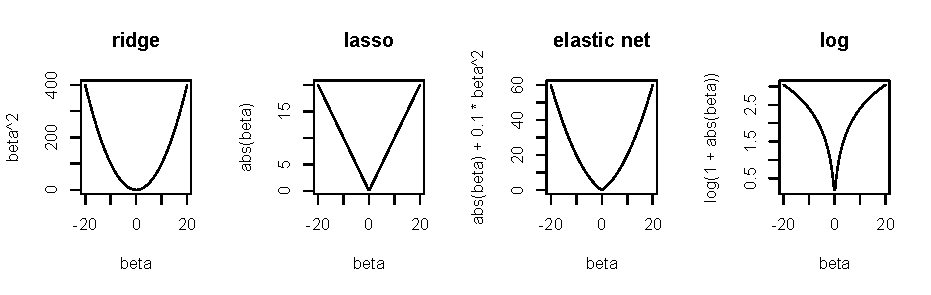
\includegraphics[width=\textwidth]{figures/penalties}
\caption{\label{costs} 
From left to right, 
$L_2$ `ridge' costs \cite{hoerl_ridge_1970}, $L_1$ `lasso' \cite{tibshirani_regression_1996}, the `elastic net' mixture of $L_1$ and $L_2$ \cite{zou_regularization_2005}, and the log penalty \cite{candes_enhancing_2008}.
}
\end{figure}

In this article we focus on the $L_1$ penalty for its balance between
shrinkage of large signals (players tend not to have huge effects) and a
preference for sparsity (we can only measure the nonzero effects of a subset
of players).  For these and many appealing theoretical reasons (and for
computational tractability), the $L_1$ penalty is by far the most commonly
used in contemporary regularized regression; see
\cite{hastie:tibsh:fried:2001} for a broad-audience overview and
\cite{taddy_one-step_2015} for details on the algorithms used in this chapter.
Under lasso $L_1$ penalization, estimation proceeds through optimization of
\begin{equation} \label{pendev}
l\left(\boldsymbol{\eta}; \mathbf{y}\right) + n\lambda \sum_{j=1}^p\left(|\beta_{0j}| + |\beta_{sj}|\right),
\end{equation}
The penalty size, $\lambda$, acts as a {\it squelch}: canceling noise to
focus on the true input signal. Large $\lambda$ lead to very simple  model
estimates, while as $\lambda \rightarrow 0$ we approach maximum likelihood
estimation (MLE). Since you don't know optimal $\lambda$, practical
application of penalized estimation requires a {\it regularization path}: a $p
\times T$ field of $\boldsymbol{\hat\beta}$ estimates obtained while moving
from high to low penalization along $\lambda^1 > \lambda^2 \ldots >
\lambda^T$. These paths begin at $\lambda^1$ set to infimum $\lambda$ such
that (\ref{pendev}) is minimized at $\boldsymbol{\hat\beta} = \mathbf{0}$, and proceed
down to some pre-specified $\lambda^T$ (e.g., $\lambda^T= 0.01\lambda^1$).

 A common tool for choosing the optimal $\lambda$---that for which we report
 estimated player effects---is cross validation (CV).  In CV, the path of
 coefficients is repeatedly fit to data subsamples and used to predict the
 response on the left-out data. The $\lambda$ leading to minimum error is then
 selected as optimal.  In this chapter, we instead use an analytic alternative
 to CV that yields models that perform as well or better out-of-sample.   The
 corrected Akaike Information Criterion (AICc), proposed in
 \cite{hurvich_regression_1989}, is defined as
\begin{equation*}
AICc = 2\sum_{i=1}^{n} l(\boldsymbol{\hat\eta}_{\lambda};\mathbf{y}) + \frac{2kn}{n-k-1},
\end{equation*}
where $\boldsymbol{\hat\eta}_{\lambda}$ are the estimated log odds under
penalty $\lambda$ and $k$ is the number of non-zero estimated coefficients at
this penalty. See \cite{taddy_one-step_2015} and \cite{flynn_efficiency_2013}
for details on AICc selection in this context; we find AICc preferable to CV
because it is computationally effecient (you only need to optimize once) and
because there is no random Monte Carlo variation---it always gives the same
answer on the same data.  However, all of our ideas here apply if you wish to
use CV selection instead. Regardless, the {\tt gamlr} package \cite{gamlr} can
be called via {\sf R} to implement this procedure:
\begin{verbatim}
R> fit <- gamlr(X, Y, standardize=FALSE, family="binomial")
\end{verbatim}
For CV, just replace \verb!gamlr! with \verb!cv.gamlr!. The
\verb!standardize=FALSE! flag tells \verb!gamlr! to \textit{not} weight the
coefficient penalties by the standard deviation of the corresponding covariate
(i.e., to use penalty $\lambda|\beta_j|$ instead of
$\lambda\mathrm{sd}(\mathbf{x}_j)|\beta_j|$); this is appropriate here because
such standardization would \textit{up-weight} the influence of players who
rarely play (and have low $\mathrm{sd}(\mathbf{x}_j)$) relative to those who
have a lot of ice time (and thus high $\mathrm{sd}(\mathbf{x}_j)$).  The
software exploits sparsity in our player effects (\verb!X!) via the
\verb!Matrix! library for {\sf R}, and is extremely fast to run: no examples
in this article require more than a few seconds of computation. Estimated
coefficients at optimal $\lambda$ are available as \verb!coef(fit)!.


One natural way to understand regularized regression is through the lens of
Bayesian posterior inference. Judiciously chosen prior distributions lend
stability to the fitted model, which is crucial in contexts where the number
of quantities being estimated is large. In our setting where larger
$\beta$-values indicate large positive or negative contributions to player
ability, it makes sense to choose a prior that encourages coefficients to
center around zero, a so-called {\em shrinkage} prior.  Our {\em a priori}
belief is that most players are members of the rank-and-file: their
contribution to goals is {\em neutral} (e.g., zero on the log-odds scale), and
that only a handful of stars (and liabilities) have a strong contribution to
the chances of scoring (or letting in) goals.  From the perspective of point
estimation on $\beta_j$ centered at zero, say, is equivalent to adding a
penalty term for $\beta_k \ne 0$ in an an objective function that is being
optimized to give us point-estimates for each $\beta_j$.

Different choices of priors correspond to different penalty functions on
$\beta_j \ne 0$. One common strategy uses a normal prior distribution
(centered at zero) on each $\beta_j$ which corresponds to a L2 penalty in the
objective function.  Thus, the {\em maximum a posteriori} (MAP) estimates from
a Bayesian regression model with a normal prior distribution are equivalent to
the estimates from ridge regression \cite{HoeKen70}. Another popular strategy
uses a Laplace prior distribution on each $\beta_j$ which corresponds to a L1
penalty ($\lambda_j |\beta_j|$) in the objective function.  Thus, the MAP
estimates from a Bayesian regression model with a Laplace prior distribution
are equivalent to the estimates from {\it lasso} regression \cite{Tib96}.  A
Laplace prior distribution yields a penalized point estimate of exactly
$\beta_j=0$ in the absence of strong evidence, and non-zero $\beta_j$ for only
a subset of significant variables.  In this way, using an L1 penalty naturally
permits {\it variable selection} where only a subset of covariates are
selected as having substantive predictive effects on the outcome variable.
Using AICc for penalty selection provides a sort of empirical Bayesian procedure: we are using prior penalization, but tuning that penalty to be optimal in prediction.


\section{Analysis: goal-based effects}
\label{sec:goals}


This section attempts to quantify the
performance of hockey players.  It extends  analysis in
\cite{gramacy:jensen:taddy:2013}.  The current version includes data about who
was on the ice for every goal in the National Hockey League (NHL) back to the
2002-2003 season, including playoffs.  The data
are in the {\tt gamlr} package; there are
69449 goals and 2439 players.

In their
initial analysis, \cite{gramacy:jensen:taddy:2013} considered even-strength
regulation-time goals data from four regular seasons, 2007--2008 during
with there were $n_p = 1467$ players involved in $n_g = 18,\!154$ goals.  The
data was obtained from \verb!www.nhl.com! via the {\sf R} package {\tt
nhlscrapr} \cite{nhlscrapr}. One problem is that the design matrix $X$ is
extremely sparse. The overall dimensions are $18,\!154 \times 1467$, which is
not overly big by modern logistic regression standards, however every row
has 1455 zeros, for more than 99\% sparsity, and the distribution of non-zero
entries is highly imbalanced: only about 27-thousand of the great than
one-million possible player papers are actually observed in the design.  


This section provides an example using data from National Hockey League, to illustrate the methodologies given in the above sections. We start by an analysis on the overall performance of players measured in goals over $11$ seasons, with an extension of the base model eq. \eqref{sec:base} by incorporating the teams and special teams effects. Furthermore, we add season effects, playoff indicators and their interactions with the players and teams. This enables us to investigate the performance of players in each season and the playoffs. We use the partial plus-minus metric to evaluate player's performance and compare that with the traditional plus-minus statistic.

We then explore an analysis based on shots instead of goals. Comparing with goals, shots are considered to be more representative in measuring the player's puck possession, and hence can hopefully provide better estimates of the player's performance. Corsi and Fenwick are two shot-based measurements that appear frequently in modern hockey analysis. Fenwick includes the shots on goal and missed shots, while Corsi measures the same thing as Fenwick but includes blocked shots. Both indicators expand our data by an order of magnitude. We compare the player's performance measured via Corsi and Fenwick with the performance in goals.

Finally, we investigate how the player's salary correlates with his performance measured via goals, Corsi and Fenwick.

The data, downloaded from \url{http://www.nhl.com}, comprise of play-by-play NHL game data for regular and playoff games during $11$ seasons of 2002-2003 through 2013-2014\footnote{Season 2004-2005 was a lockout that resulted in a cancellation}. The data capture all the shifts in every single game, such as change, goal, shot, blocked shot, miss shot, penalty and etc. There were $n_p=2439$ players involved in $n_g=69449$ goals, $n_p=2566$ players involved in $n_{cos}=1,329,679$ Corsi and $n_p=2564$ players involved in $n_{fen}=1,034,154$ Fenwick.

It is not unusual to have penalties or non-six-on-six situations in hockey. There are more than $35\%$ of the $n_g=69449$ goals fit in the power-play situations, which inspires us to incorporate the special teams in our base model eq.\eqref{eq:model}. We consider $6$ non-six-on-six settings (6v5, 6v4, 6v3, 5v4, 5v3, 4v3) and pulling the goalie together to form $7$ different special teams situations. Meanwhile, to reduce the effect of teammates on the player's performance, we add team indicators to the base model as well.


The seasonal data are aggregated and arranged into a response vector $\vec{Y}(n_g \times 1)$ and a design matrix $\vec{X}$. The design matrix comprises of three parts, $X_P(n_g\times n_p)$, $X_T(n_g\times 30)$ and $X_S(n_g\times 7)$, which correspond to indicators of players, teams and special teams respectively. For a goal $i$, the response can either take value $y_i=1$ for goal scored by the home team or $y_i={-1}$ for it scored by the away team. The corresponding row of $X_P$, $X_T$ represents the players and teams on the ice for that goal, with value $1$ for home player/team, ${-1}$ for the away player/team and $0$ otherwise. As to the special-team indicator $X_S$, $X_{Sij}=1$ indicates the home team is experiencing the $j$th special-team status while $X_{Sij}=-1$ indicates the away team is playing with the $j$th status. 

\subsubsection{Mapping from player coefficients to the plus-minus scale.}
\label{sec:ppm.mapping}
Note that the player effect $\beta_i$ corresponds to a per-goal scale, which is the log odds that a given goal was scored by their own team. It is incomparable with the traditional plus-minus due to the difference of scales. We consider a partial plus-minus statistic (PPM) by incorporating the number of games that a player played in addition to the per-goal effect. Denote $G_i$ as the number of goals that a player was on the ice for. Then given a player effect $\beta_i$, we calculate the probability that, given a goal was scored, it was scored by his own team as $P_i=1/(1+exp(-\beta_i))$. The PPM is the expected contribution to the goal differential due to that player, which is 
\begin{equation}
\text{PPM}_i = G_iP_i-G_i(1-P_i)=G_i(2P_i-1).
\label{eq:ppm}
\end{equation}

We can see the correspondence of the player effect and the PPM. The PPM only scales the player effect with the sign retains. This means that if a player has a positive effect, $\beta_i>0$, its corresponding PPM is also positive. 


 
\subsection{Point estimates of player contribution via goals}
%%% code:  performance_sen_goal.R
\subsubsection{Team effects}
We first ignore the special-team effect and consider two models for conditional player effect estimation: a player-only model and a team-player model. Both models have about 900 players with zero effects, resulting from the MAP estimation under a sparsity-inducing L1 penalty. Note that ability estimates for players who frequently share the ice will generally be negatively correlated: if players are always on the ice together when a goal is scored, an increase in the estimated effect of one player must be accompanied by a decrease in the fact of the other player. And the L1 regularized model will manifest it by forcing one players effect being estimated at zero.

Figure \ref{fig:pt-p.tb20} shows the partial plus-minus (PPM) obtained for the team-player model under MAP estimation (dots), and compares to those from the player-only model (connecting lines). The $x$-axis orders the players by their PPM in the team-player model, expressing a marginal ordering on player ability. Only the top 20 and bottom 20 players in either model are shown. 

Observe that incorporating the team effects causes many player effects to be more significant, especially for the top players (blue lines tracking to the dots). Henrik Lundqvist, the Sweden goaltender, shines as the leagues best in both models. Meanwhile, on the negative side, Chris Phillips and Brendan Witt stands out as poor performers in either model. 

Note that incorporating the team effects does not show the signal of changing the signs of player effects. This means a player being positive in the player-only model will not be negative after accounting for his team. In this sense, the team-player model and the player-only model are pretty consistent. However, it is worth noticing that some `giant' players, such as Sidney Crosby and Pavel Datsyuk, considered by many to be the league's very best, are not in our top 20 list. This inspires us to further improve our model by incorporating the special-team effects. 

\begin{figure}[htb!]
    \centering
    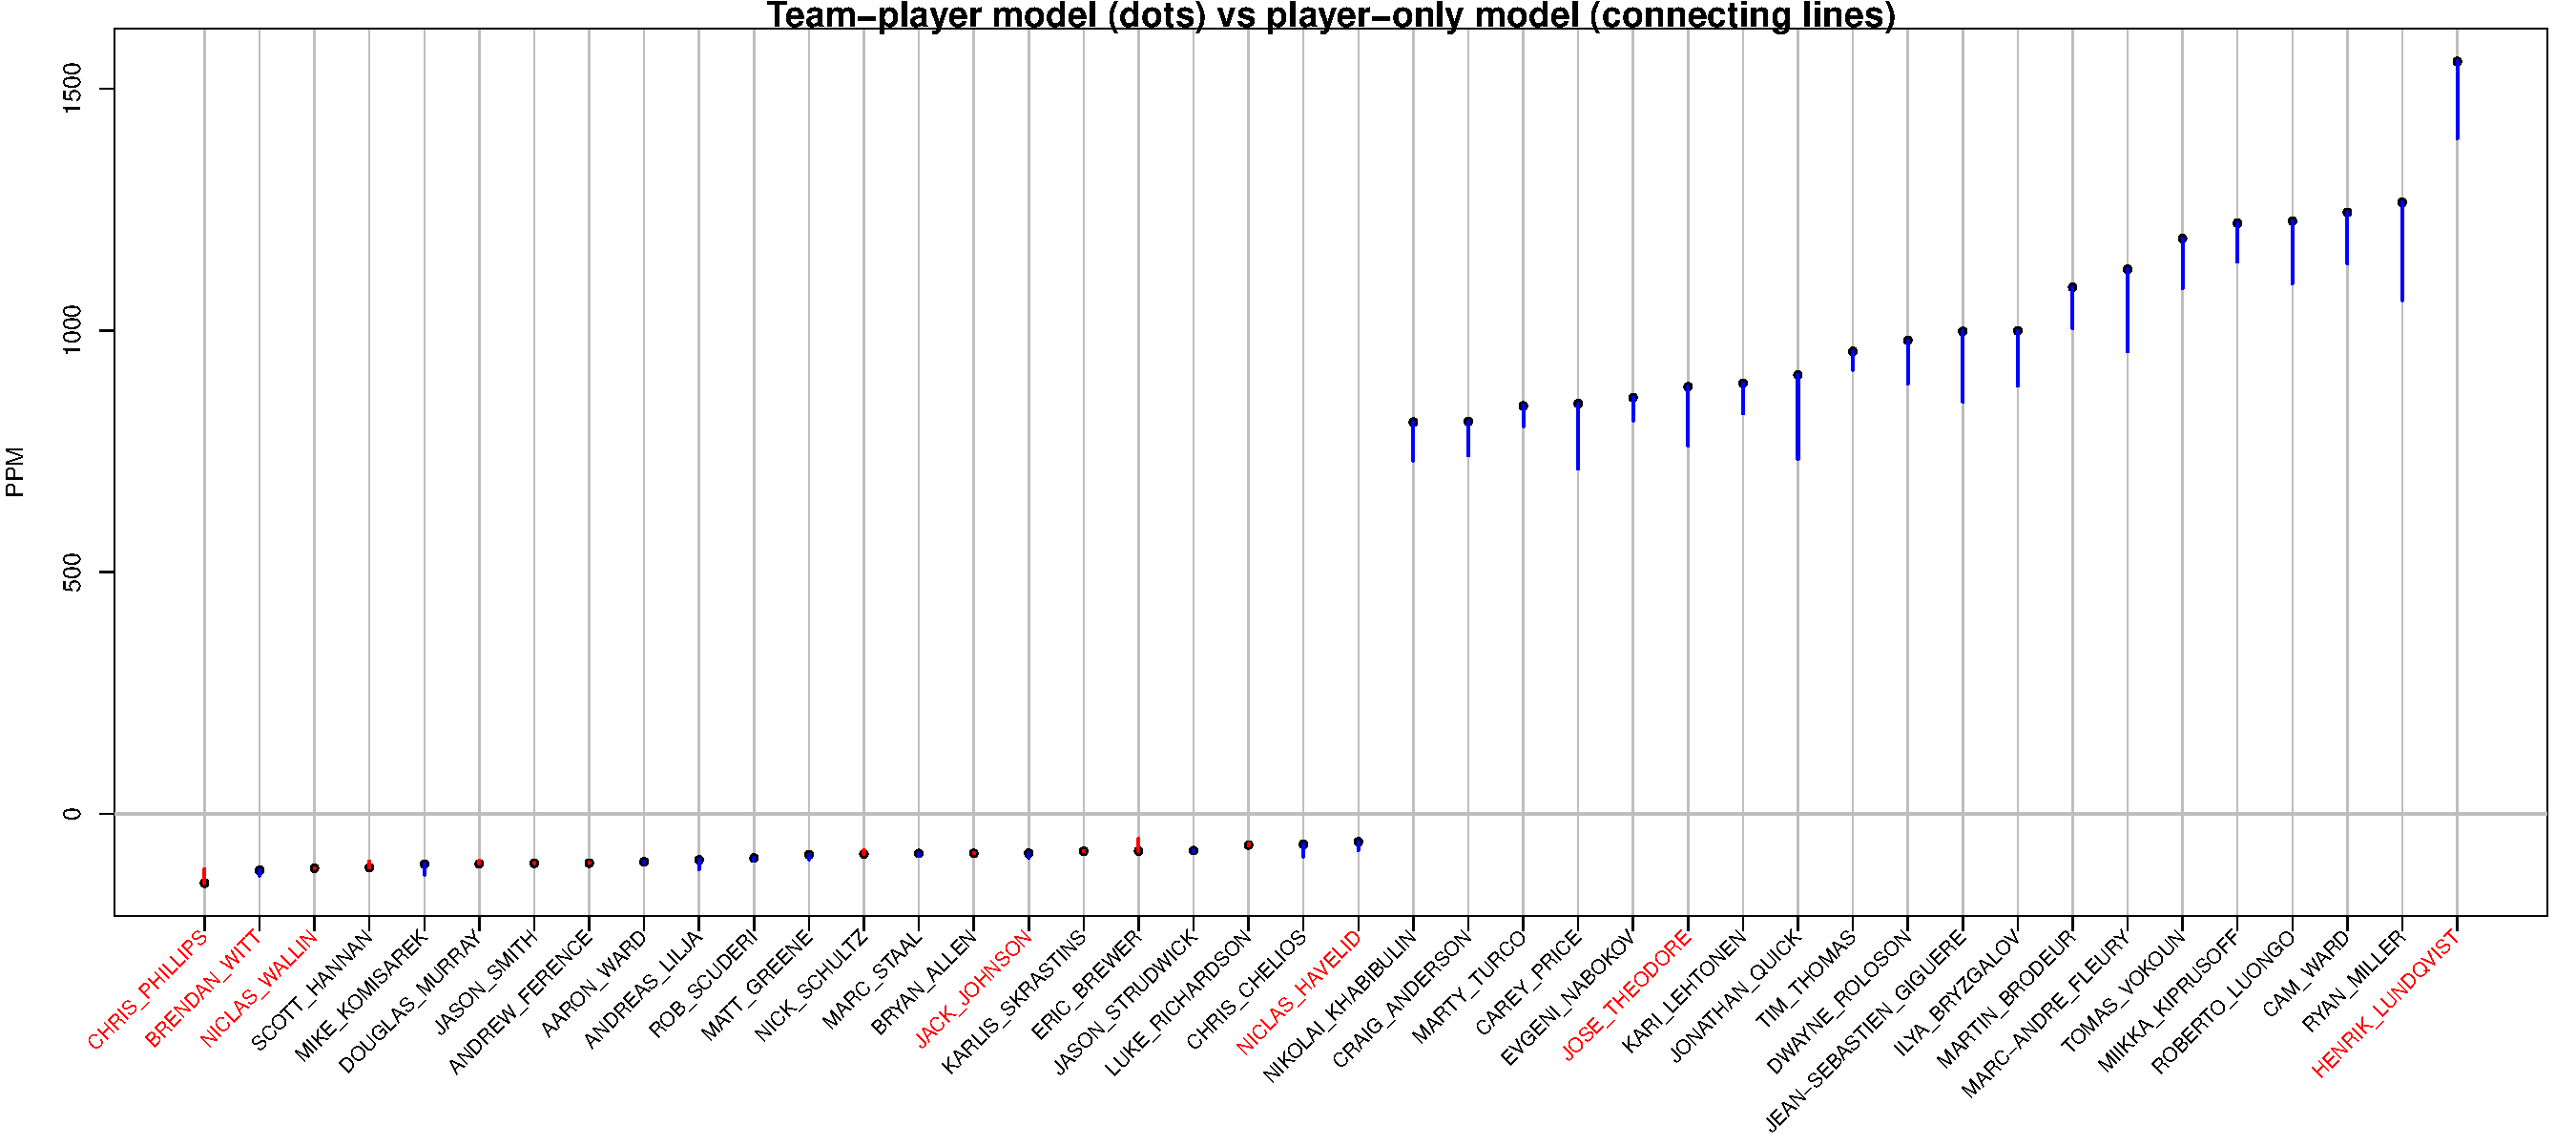
\includegraphics[width=\textwidth]{figures/ptvsp_tb20.pdf}
    \caption{Comparing the partial plus-minus (PPM) for players in the player-only model (lines), with the team-augmented model (dots). The lines point to estimated coefficients from the player-only model. We are only showing players whose PPM are top 20 or bottom 20 in either model. Players discussed in the text have their names labeled in red.}\label{fig:pt-p.tb20}
\end{figure}

\subsubsection{Special-team effects}
Now we add the special-team effects to form the model \eqref{eq:modelwithL2}, and compare it with the team-player model. Figure \ref{fig:pts-pt.tb20} shows the partial plus-minus (PPM) obtained for both models. One fact is that employing the special-team effects makes many more player effects to be zeroed out (lines tracking to zero), with many players' stand-out performance being absorbed by the power-plays. In another words, a short-handed goal will be a big 'plus' to the players on the ice of the short-handed team, and a big 'minus' to the opponent players. 

A more surprising result is that, incorporating the special-team effects causes many changes in the signs of player effects, which does not happen in the team-player and player-only comparison. An example is Jose Theodore, whose contribution drops significantly from positive to negative after accounting for the power plays. Patrick Lalime has the similar behavior and becomes one of the bottom players.

Most of the top and bottom players are now consistent with expectations. Marian Hossa stands out as the best player in the league, followed by Sidney Crosby. Henrik Lundqvist remains to be top despite the large drop of his contribution. 

Table \ref{tab:goal.ppm.rank} shows the statistics of the top and bottom six players. For percentage (FP), in the table, is another metric used in many modern Hockey analytics. Goals are counted as 'For' or 'Against', where 'For' is a goal that is scored when the player is on the ice on behalf of his team and 'Against' is a goal by his opponents. 'FP' is then given as a percentage of $\text{For}/(\text{For}+\text{Against})$. Note that the plus-minus statistic is just $\text{For}-\text{Against}$. 

Some interesting trends can be pointed out here. First, forwards dominate the top of the list while the bottom players tend more likely to be defenders. This is not unexpected since ... (an explanation here). Meanwhile, PPM an PM are consistent in the signs except for Patrick Lalime, who has a positive PM but a large negative PPM. Finally, players can hardly be distinguished using for percentage (FP). All the top 6 players have very similar FP while their PPM ranges from $277.80$ to $348.33$. 

Herik Sedin, ranked 6th according to the table, captains the Vancouver Canucks and became the all-time leading scorer for the Canucks in 2013. The Swedish center scored 10 goals and 71 assists in 82 regular games of season 2006-2007. However, in 2007 playoffs, he was on the ice for twelve games but only scored two goals and two assists. As our player-special team-team model only evaluates the overall performance of players, such phenomenon can not be spotted. 

\begin{figure}[htb!]
    \centering
    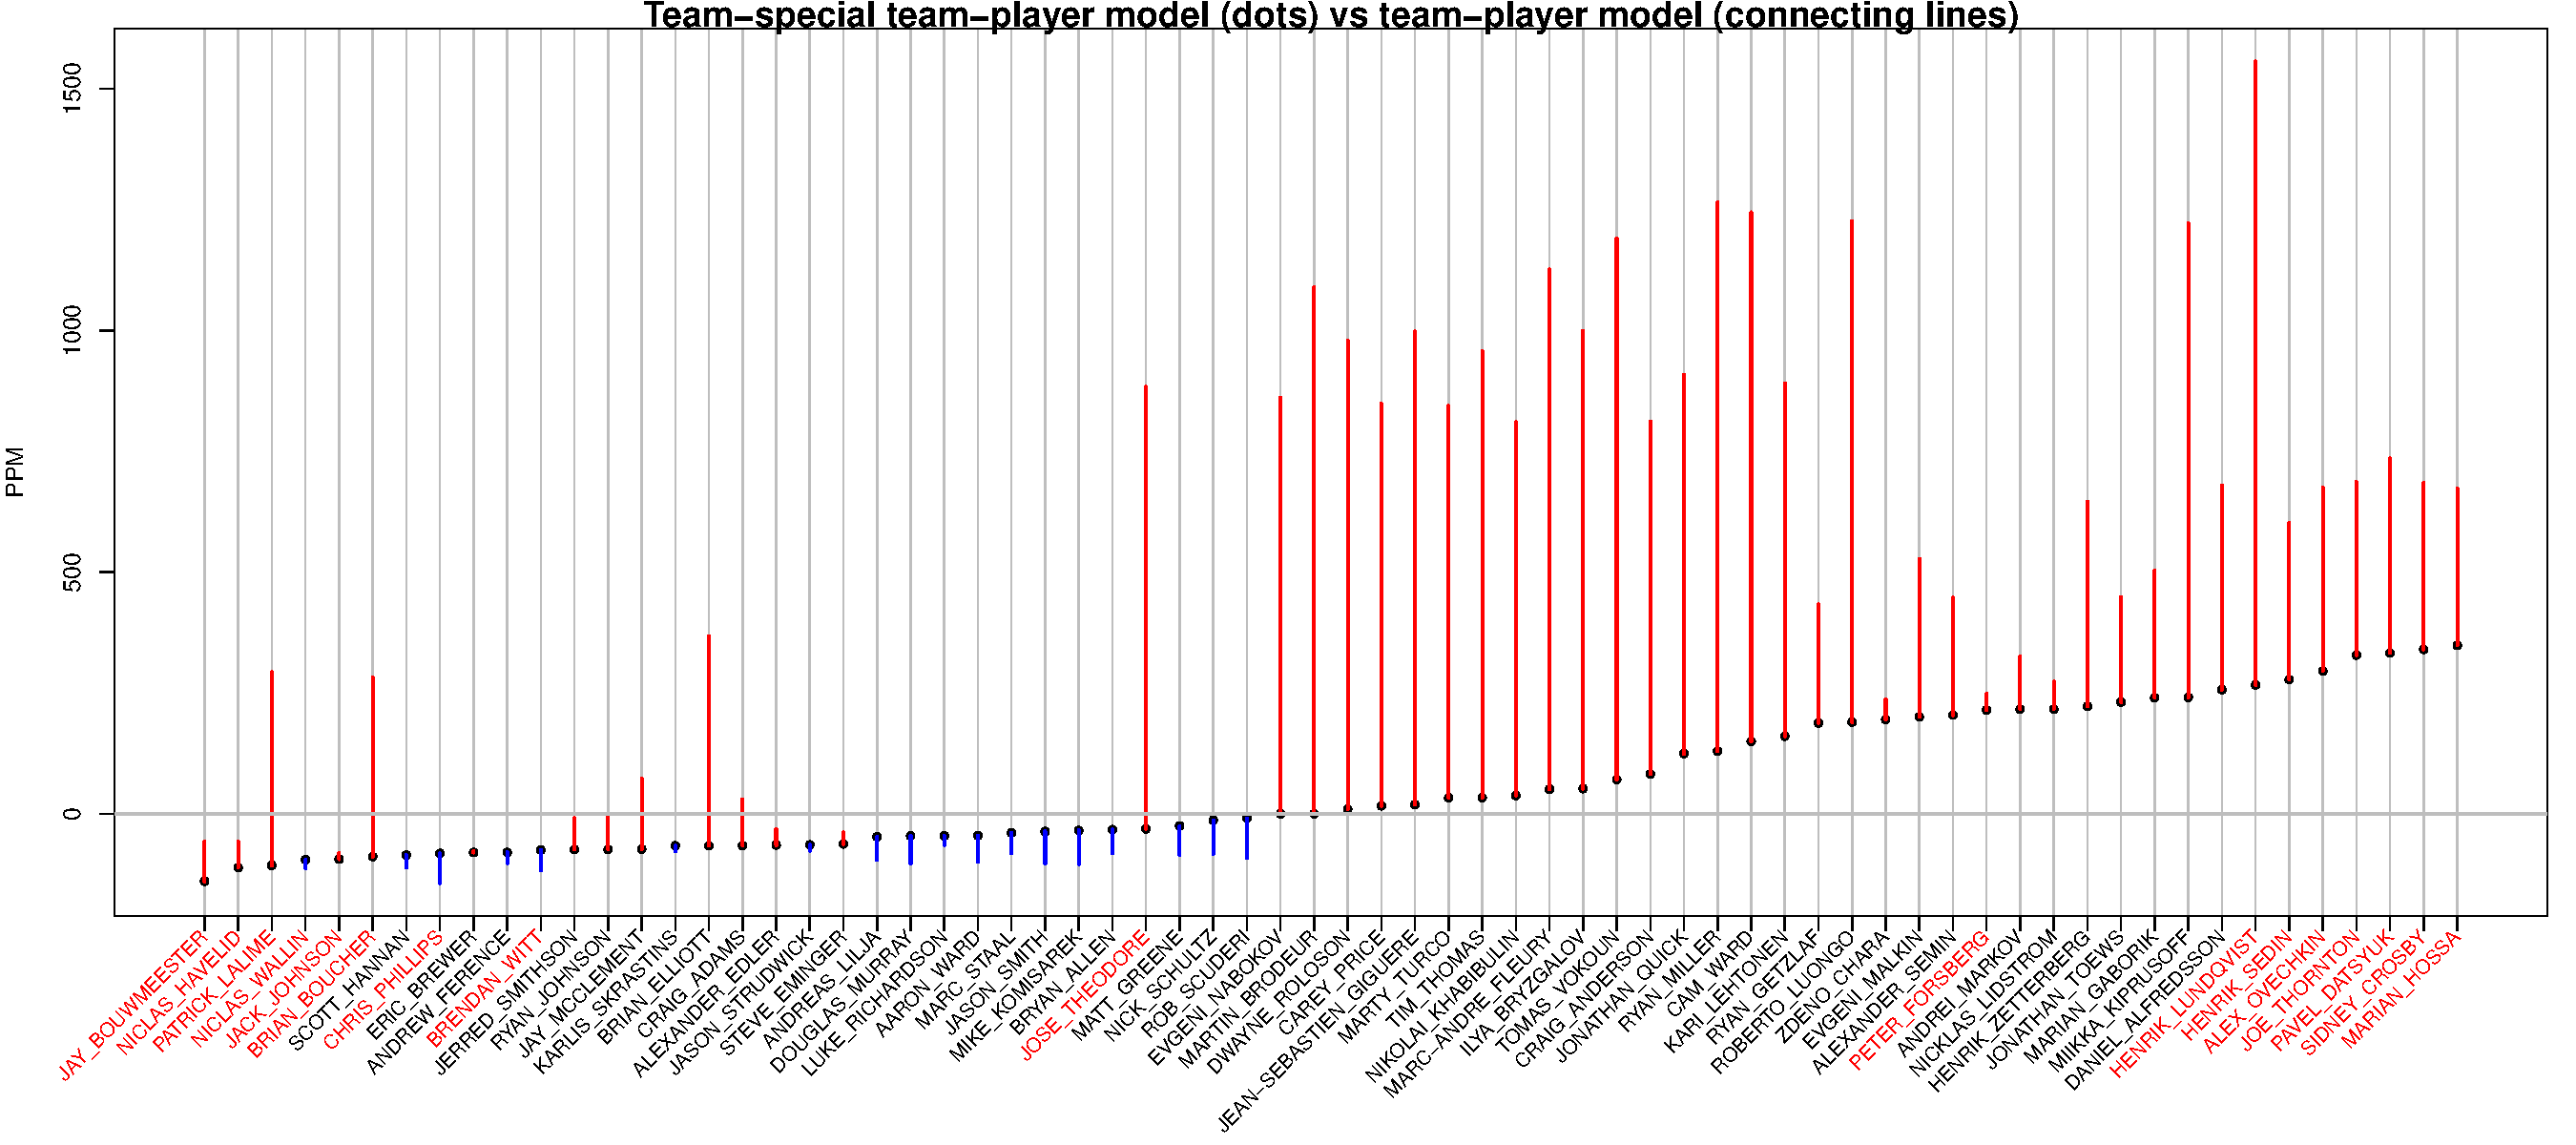
\includegraphics[width=\textwidth]{figures/ptsvspt_tb20.pdf}
    \caption{Comparing the partial plus-minus (PPM) for players in the team-player model (lines), with the team-special team-player model (dots). The lines point to estimated coefficients from the team-player model. The $x$-axis orders the players by their estimates in the team-special team-player model. We are only showing players whose PPM are top 20 or bottom 20 in either model.}\label{fig:pts-pt.tb20}
\end{figure}

{
    \renewcommand{\arraystretch}{1.2}
    \begin{table}[htbp]
        \centering
        \begin{tabular}{r c c r r r r r }
            \hline
            Rk & Player & Pos & G & Beta & \textbf{PPM} & PM & FP \\ \hline
            1 & MARIAN HOSSA            & R & $1752$ & $0.40$ & $348.43$ & $448$ & $0.63$ \\
            2 & SIDNEY CROSBY          & C &  $1568$ & $0.44$ & $340.09$ & $544$ & $0.67$ \\
            3 & PAVEL DATSYUK          & C &  $1725$ & $0.39$ & $332.62$ & $\mathbf{599}$ & $0.67$ \\
            4 & JOE THORNTON            & C & $1740$ & $0.38$ & $328.30$ & $510$ & $0.65$ \\
            5 & ALEX OVECHKIN           & L &  $1705$ & $0.35$ &$295.34$ & $533$ & $0.66$ \\ 
            6 & HENRIK SEDIN   & C & $1634$ & $ 0.34$ & $277.80$ & $542$ & $0.67$ \\ \hline
            2434 & BRIAN BOUCHER   & G & $1059$ & $-0.17$ & $-88.57$  & $-87$ & $0.46$ \\
            2435 &  JACK JOHNSON        & D  & $990$ & $-0.19$ & $ -93.84$ & $-54$ & $ 0.47$\\
            2436 &  NICLAS WALLIN           & D  & $764$ & $-0.25$ & $ -94.95$ & $-170$ & $ 0.39$\\
            2437 &  PATRICK LALIME          & G & $1240$ & $-0.17$ & $ -106.68$ & $ 22$ & $ 0.51$\\
            2438 & NICLAS HAVELID       & D & $1041$ & $-0.21$ & $ -111.20$ & $-131$ & $ 0.44 $\\
            2439 &  JAY BOUWMEESTER         & D & $1870$ & $-0.15$ & $ -139.59$ & $-142$ & $ 0.46$\\ \hline
        \end{tabular}
        \caption{Top 6 and bottom 6 players in partial plus-minus (PPM), obtained from the team-special team-player model. 'Pos' is the position of the player (center, left wing, right wing, defenseman, goaltender). 'G' is the number of goals that the player has involved. 'Beta' is the player effect from the regression model. 'PPM' and 'PM' are the partial-plus minus and traditional plus-minus statistics respectively. 'FP' is the for percentage.  }\label{tab:goal.ppm.rank}
    \end{table}
}

\subsubsection{Season-playoff effect}
We consider the two more features, the playoffs (dummy variable, equals to $1$ if the goal is scored in playoffs and $0$ if it is in the regular session) and seasons (dummy variable, with $1$ indicating the season when the goal was scored). A heuristic way of writing model \eqref{eq:model.ext} is given as
\begin{equation*}
\text{logit(goal)} =  \vec{\beta_P}^\prime \text{player} + \vec{\beta_T}^\prime \text{team} + \vec{\beta_S}^\prime \text{special-team}.
\end{equation*}
We now incorporate the interactions of seasons and playoffs with players and teams. The model can be written as
\begin{equation}
\begin{aligned}
\text{logit(goal)} = & \vec{\beta_P}^\prime \text{player} +  \vec{\beta_S}^\prime \text{special-team} + \vec{\alpha_{TS}}^\prime \text{team}:\text{season} +  \vec{\alpha_{TSP}}^\prime \text{team}:\text{season}:\text{playoff} \\
& +\vec{\alpha_{PS}}^\prime \text{player}:\text{season} +  \vec{\alpha_{PSP}}^\prime \text{player}:\text{season}:\text{playoff}   ,
\end{aligned}
\label{eq:model.inter}
\end{equation}

where  $\vec{\alpha_{PS}}$ is the coefficient of the player-season interaction, $\vec{\alpha_{PSP}}$ is the coefficient of the player-season-playoff interaction, $\vec{\alpha_{TS}}$ is the coefficient of the team-season interaction and $\vec{\alpha_{TSP}}$ is the coefficient of the team-season-playoff interaction. By imposing L1 penalties on all the coefficients related to players, $\vec{\beta_P}$, $\vec{\alpha_{PS}}$ and $\vec{\alpha_{PSP}}$, we can obtain the {\em maximum a posteriori} estimates.

Table \ref{tab:goal.ppm.ranking.inter} shows the top and bottom five players in PPM of the regular sessions across all 11 seasons. All the players in the list are quite familiar as they appeared frequently in our previous discussion. Observe that Peter Forsberg, ranks 14th overall as shown in figure \ref{fig:pts-pt.tb20}, played really well in season 20022003, indicated by the $20\%$ more PPM than the second place. Meanwhile, Sidney Crosby, appears four times in the top 10 list, is probably the most consistent player. To be notice that, his performance in 2009 playoffs actually dominates the playoff performance of all other players. Another fact is that here's no signal of players performing differently in regular sessions and playoff ($\vec{\alpha_{PSP}=\vec{0}}$). 

{
    \renewcommand{\arraystretch}{1.2}
\begin{table}[htbp]
    \centering
    \small
    \begin{tabular}{rccrrrrrr}
        \hline
        Rk    & Player & Season & Beta.Re  & \textbf{PPM}.Re  & PM.Re & Beta.Po & PPM.Po & PM.Po \\
        \hline
        1     & PETER FORSBERG & 20022003 & 0.74  & 55.52 & 85 & 0.74  & 4.6 & 5\\
        2     & SIDNEY CROSBY & 20092010 & 0.41  & 43.47 & 60 & 0.41  & 7.45 & 19\\
        3     & DOMINIK HASEK & 20052006 & 0.35  & 42.45 & 80 & 0     & 0 & 0 \\
        4     & SIDNEY CROSBY & 20082009 & 0.41  & 42.26 & 48 & 0.41  & \textbf{10.87} & 26 \\
        5     & SIDNEY CROSBY & 20052006 & 0.41  & 41.86 & 52 & 0     & 0  & 0\\
        10200 & PATRICK LALIME & 20022003 & -0.27 & -37.81& 47 & -0.27 & -8.76 & 12\\
        10201 & PATRICK LALIME & 20032004 & -0.27 & -37.81& 37 & -0.27 & -3.05 & -3\\
        10202 & NICLAS HAVELID & 20062007 & -0.67 & -62.64 & -22 & -0.67 & -3.55 & -7 \\
        10203 & NICLAS HAVELID & 20052006 & -0.7  & -65.94 & -41 & 0     & 0 & 0\\
        10204 & JAY BOUWMEESTER & 20052006 & -0.69 & -69.62 & -32 & 0     & 0 &0\\
        \hline
    \end{tabular}%
    \caption{Top 5 and bottom 5 players in partial plus-minus (PPM) of the regular sessions, obtained from the team-special team-player model with the season and playoff effects incorporated. We are showing the player effects and PPM for both the regular sessions and playoffs.}\label{tab:goal.ppm.ranking.inter}
\end{table}
}

\section{Analysis: comparison to shot-based metrics}
\label{sec:shots}

Examples in
the literature include , and indices
such as Fenwick, Corsi, or DeltaSOT, as reviewed by \cite{vol10}. 

There are many
ways of adding complexity, for example by taking into account a larger set of
game-relevant factors such as hits, faceoffs, possession, shots.   While some
of these measures are gaining in popularity, analysts do not generally agree
on the relative importance of the added information.  Most importantly, none
of these metrics offer a partial effect: .


We have seen that Henrik Sedin's worse performance in 2007 playoffs than in the regular session, can not be captured via measures in goals. In this section, we consider two ratings in shots, the Fenwick (shot plus missed shots) and the Corsi (Fenwick plus blocked shots), which are commonly used in hockey analytics due to the large amount of information these ratings cover. 

\begin{enumerate}
    \item Overall relationship. First consider the team-special team-player model without interactions. Figure \ref{fig:ppm_diffmeasure} shows the PPM under different measures. Corsi and Fenwick shows very similar results (correlation=$0.96$). 
    \item Consider the season-playoff effects. Now we can see that some players have different regular-playoff performances ($\vec{\alpha_{PSP}\neq \vec{0}}$). For example, Henrik Sedin has a player effect of $-0.11$ for the regular session of season 2006-2007 while he has a playoff-player effect of $-0.35$.
    \item Figure \ref{fig:ppm-corr-diffmeasure-season} shows the correlations over 11 seasons. 
    \item Maybe compare the top \& bottom players in goals vs shots?
\end{enumerate}

\begin{figure}[t!]
    \centering
    \begin{subfigure}[t]{0.5\textwidth}
        \centering
        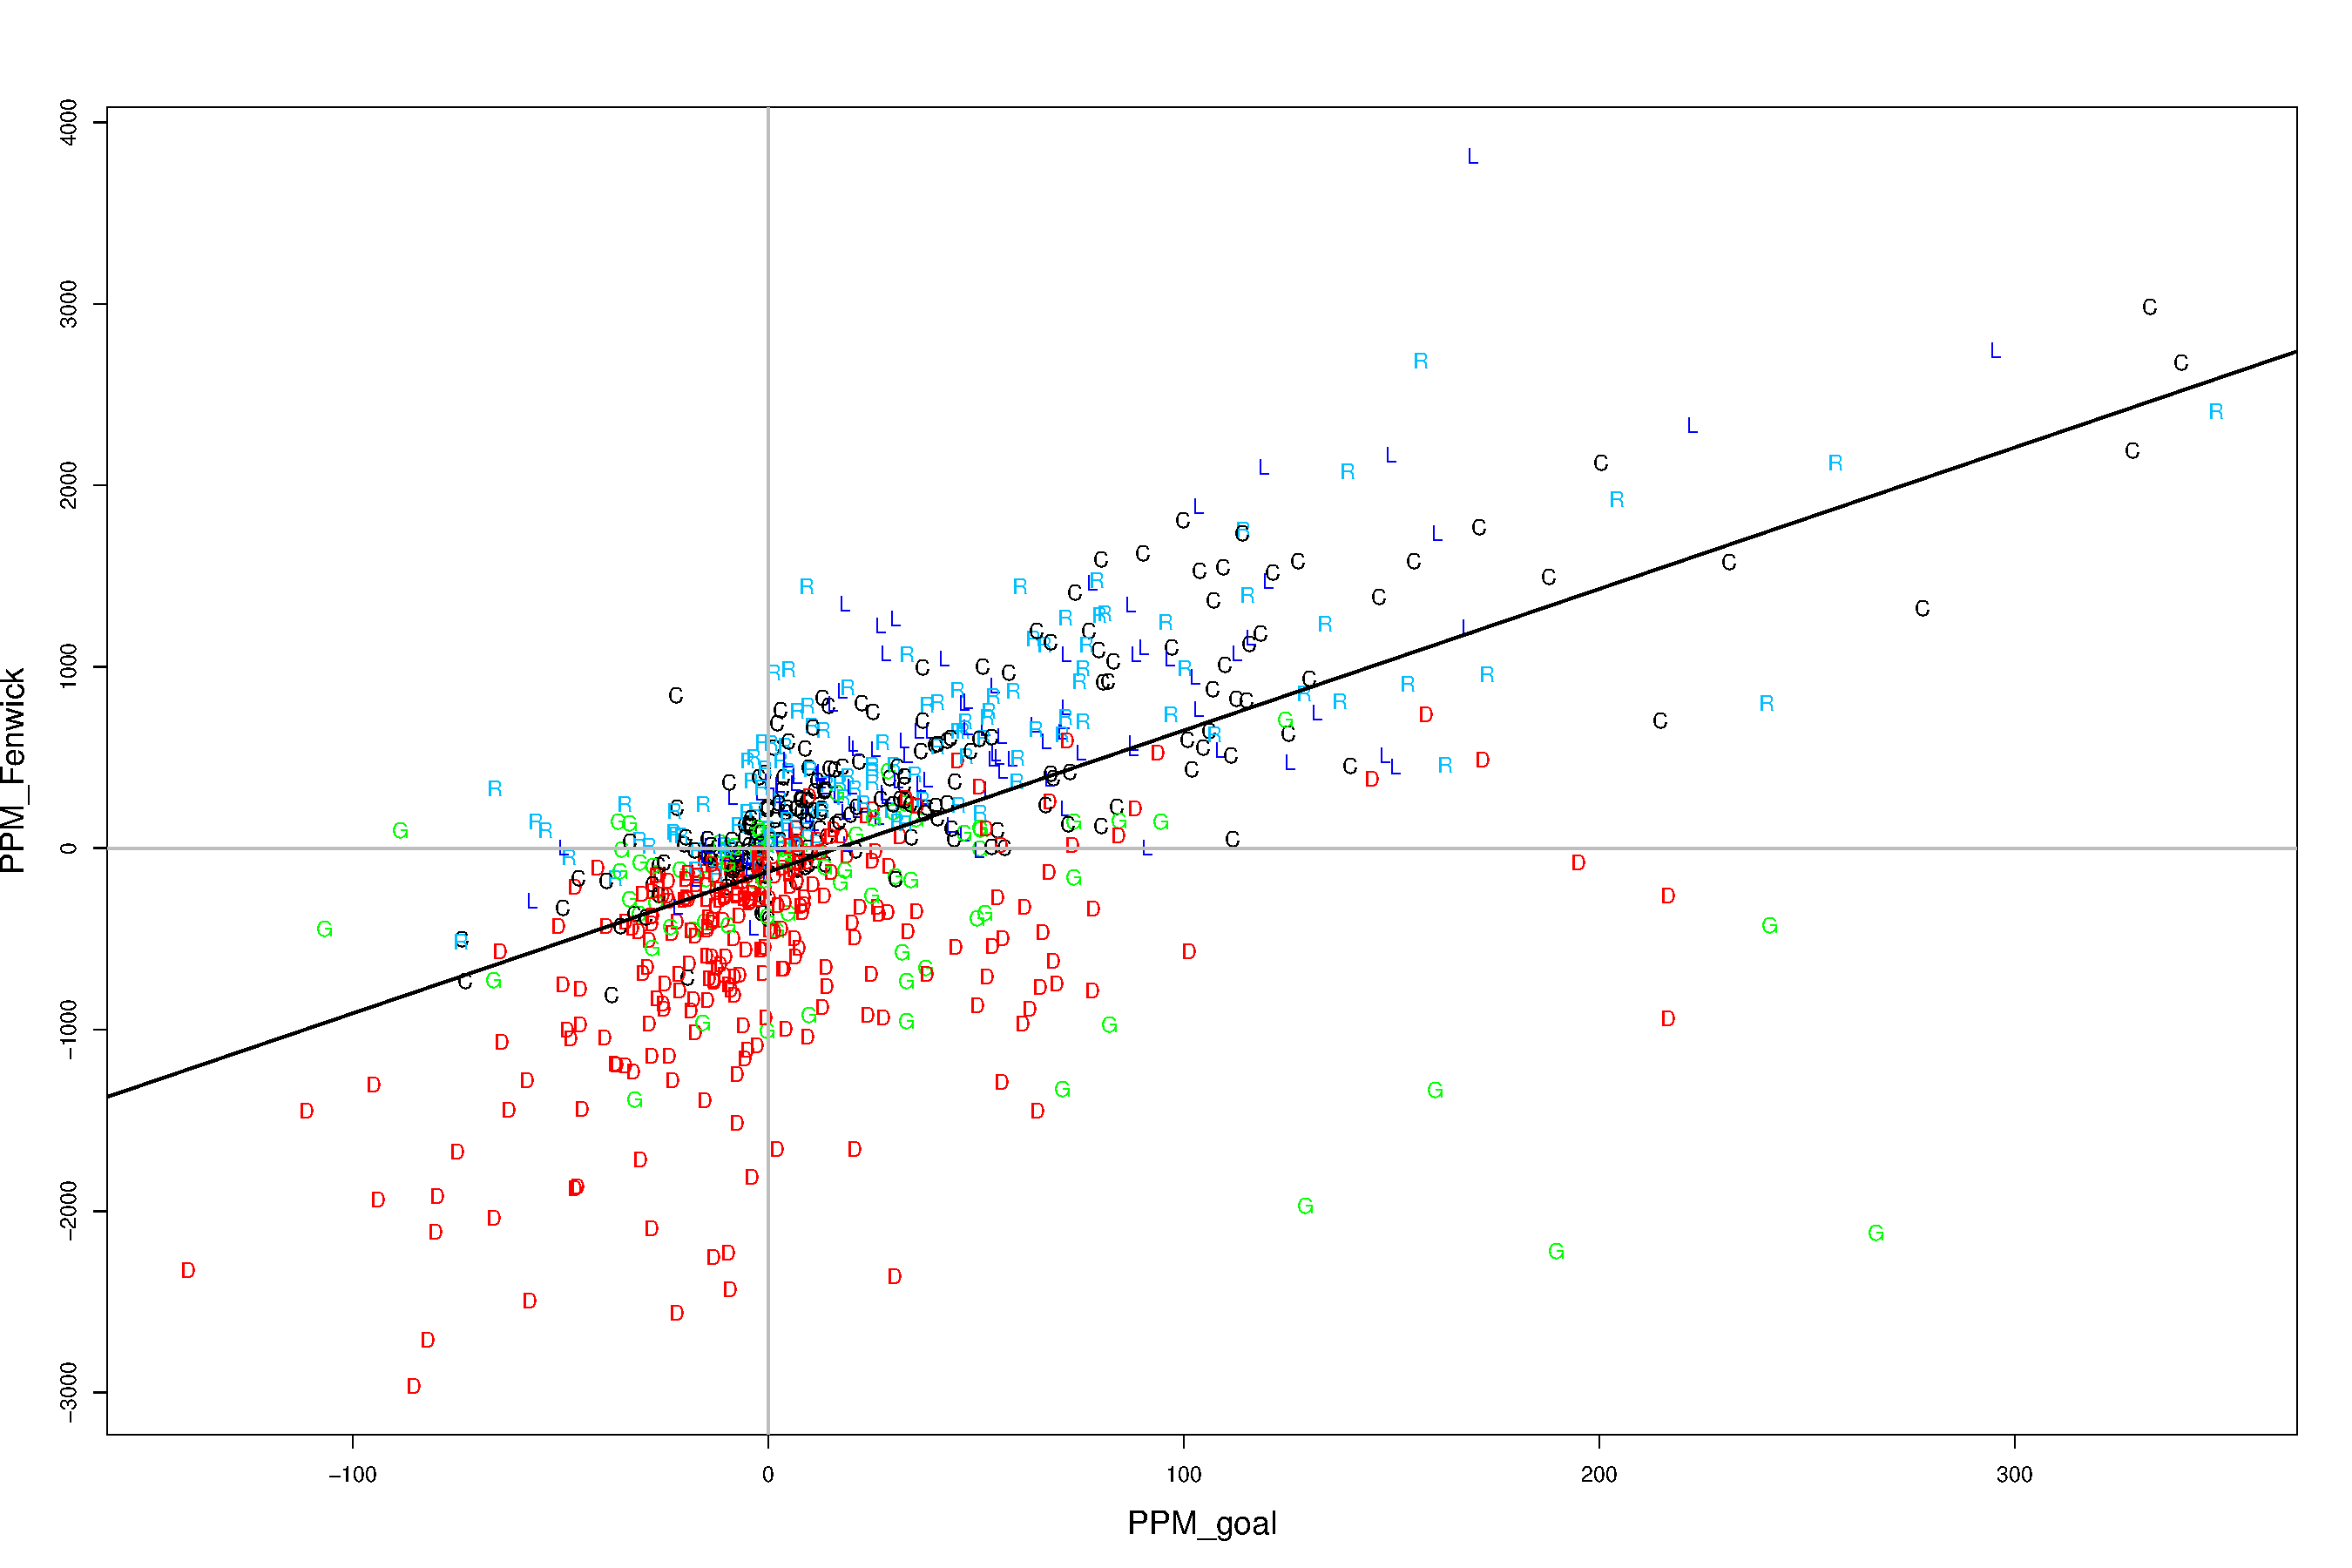
\includegraphics[height=2.2in]{figures/fenwickvsgoals_overall.pdf}
        \caption{PPM(Fenwick) vs PPM(goals)}
    \end{subfigure}%
    ~ 
    \begin{subfigure}[t]{0.5\textwidth}
        \centering
        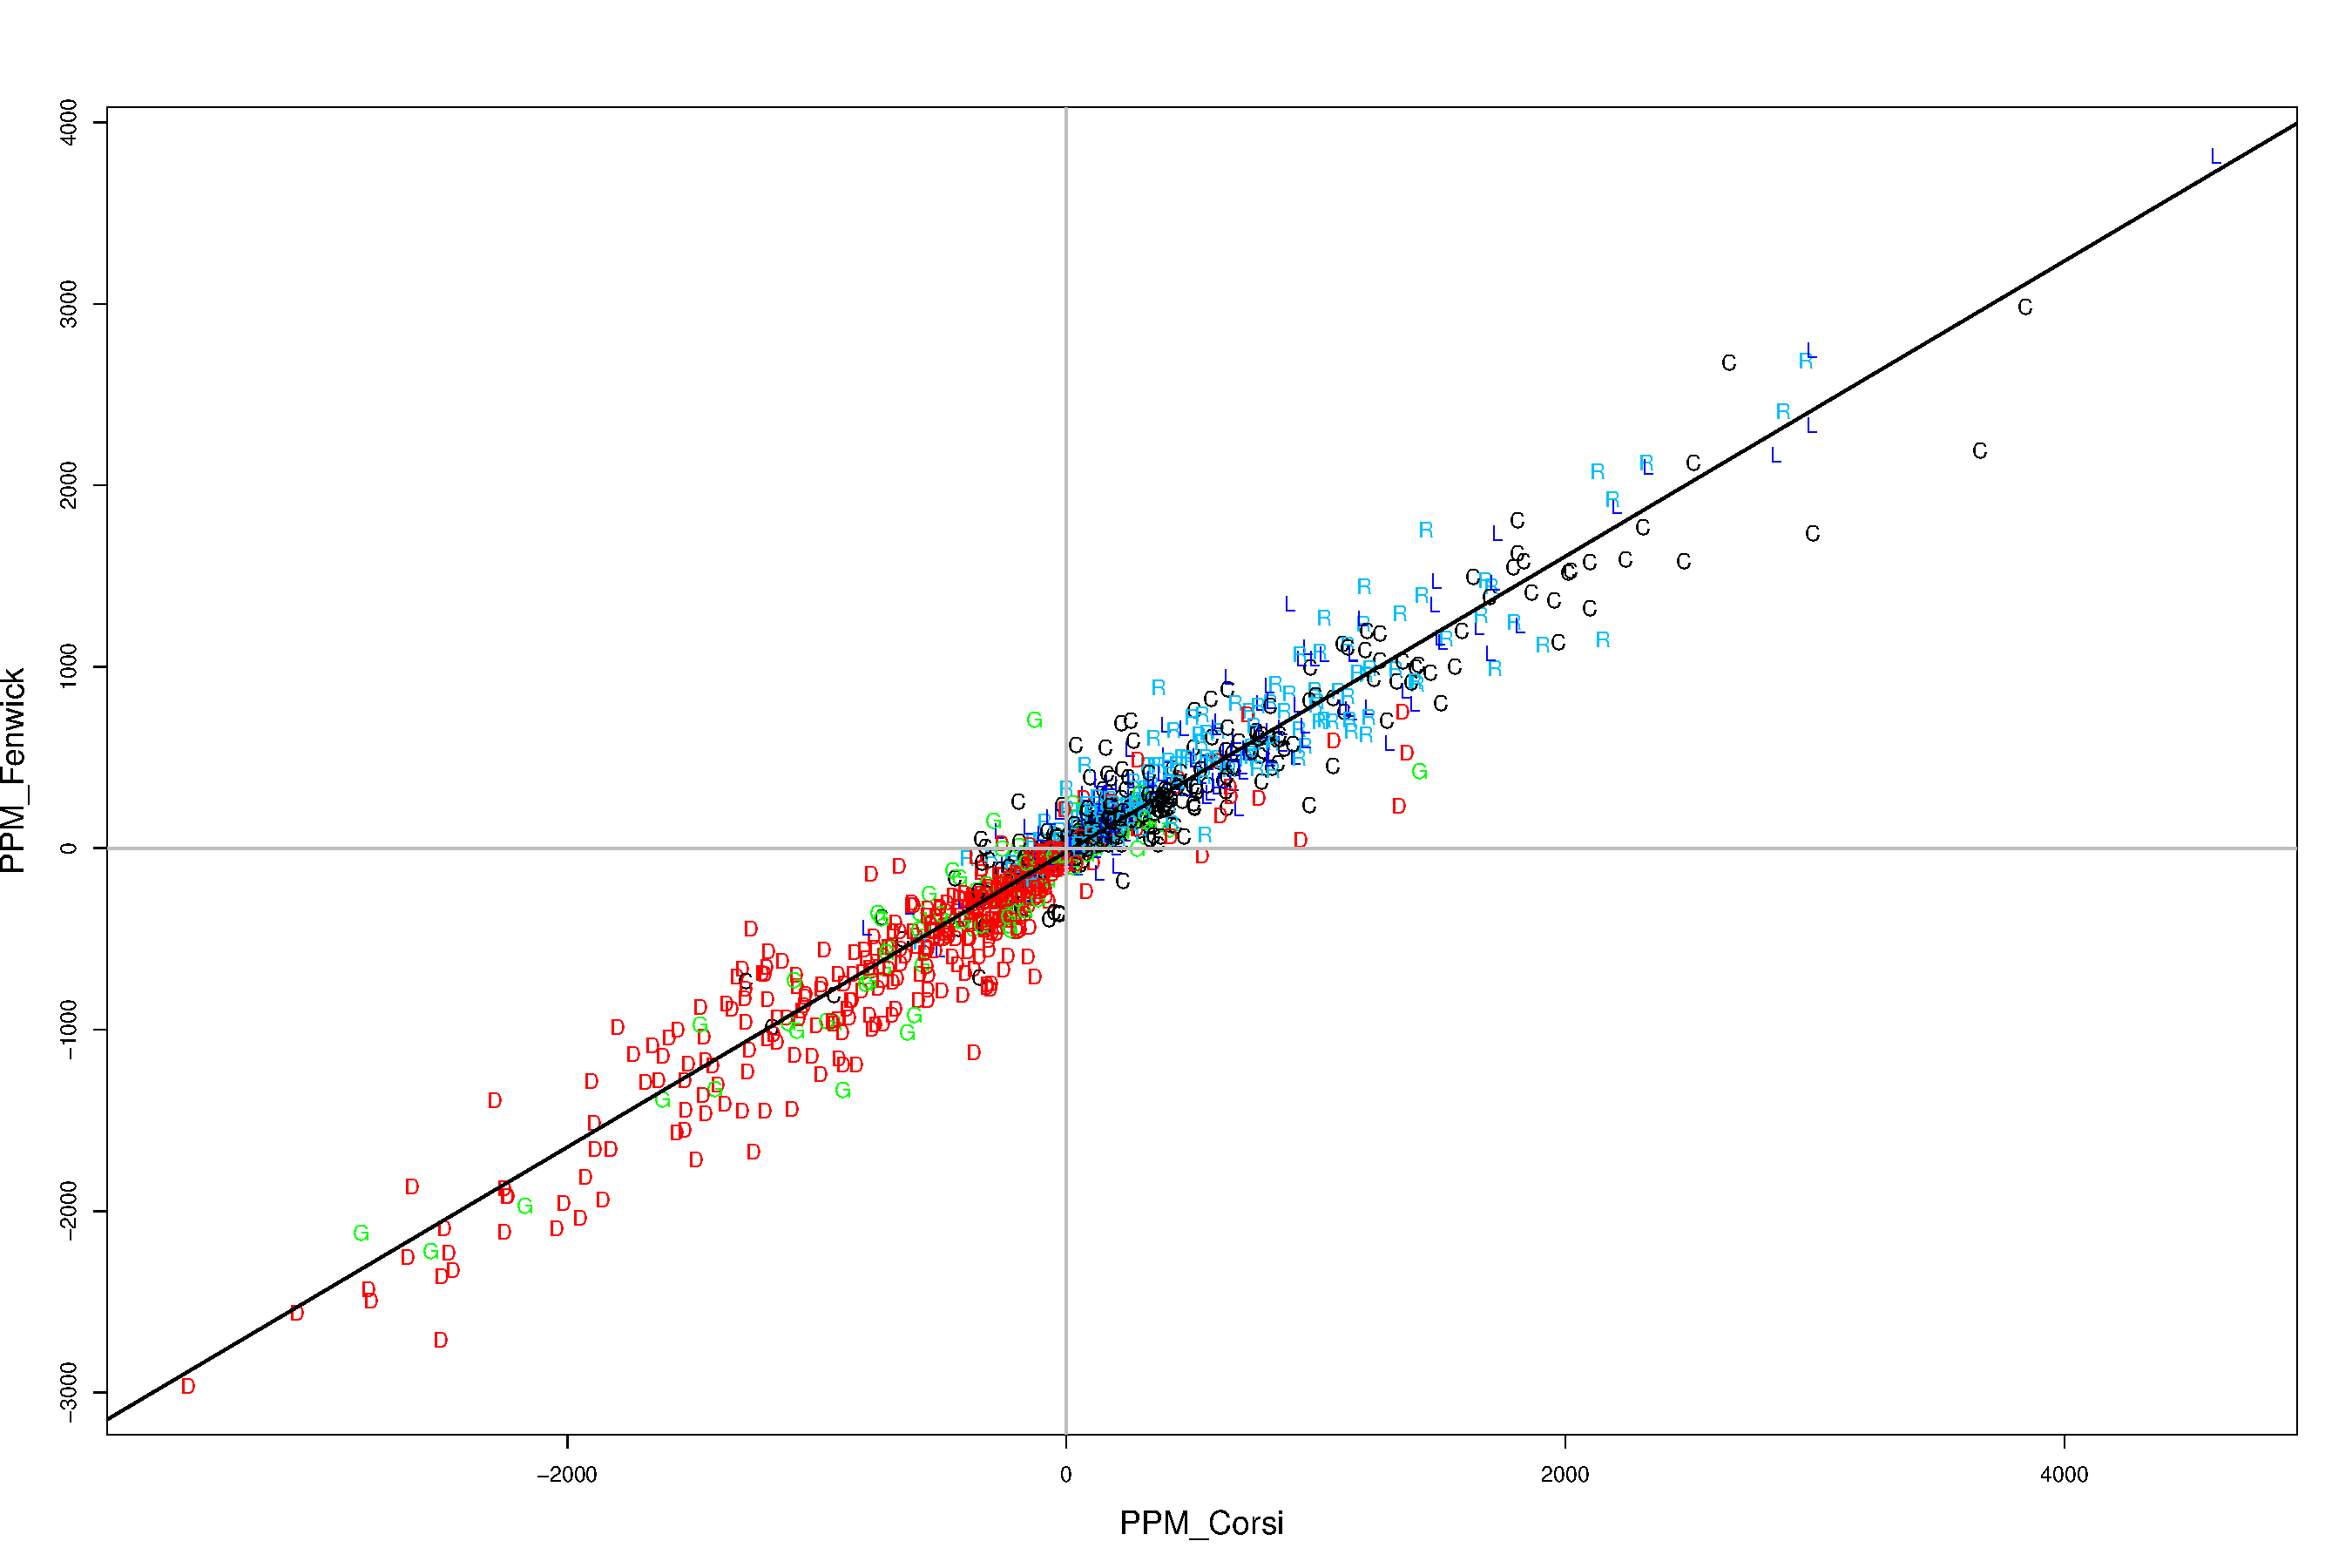
\includegraphics[height=2.2in]{figures/fenwickvscorsi_overall.pdf}
        \caption{PPM(Fenwick) vs PPM(Corsi)}
    \end{subfigure}
    \caption{Left: Comparing PPM measured via goals, to PPM measured via Fenwick (correlation=$0.54$). Right: Similarity of Corsi and Fenwick (correlation=$0.96$). Only players with non-zero PPM in either measure are shown. Plot symbols give position information, C-center, L-left wing, R-right wing, D-defense, and G-goalie.}
    \label{fig:ppm_diffmeasure}
\end{figure}

\begin{figure}[htb!]
    \centering
    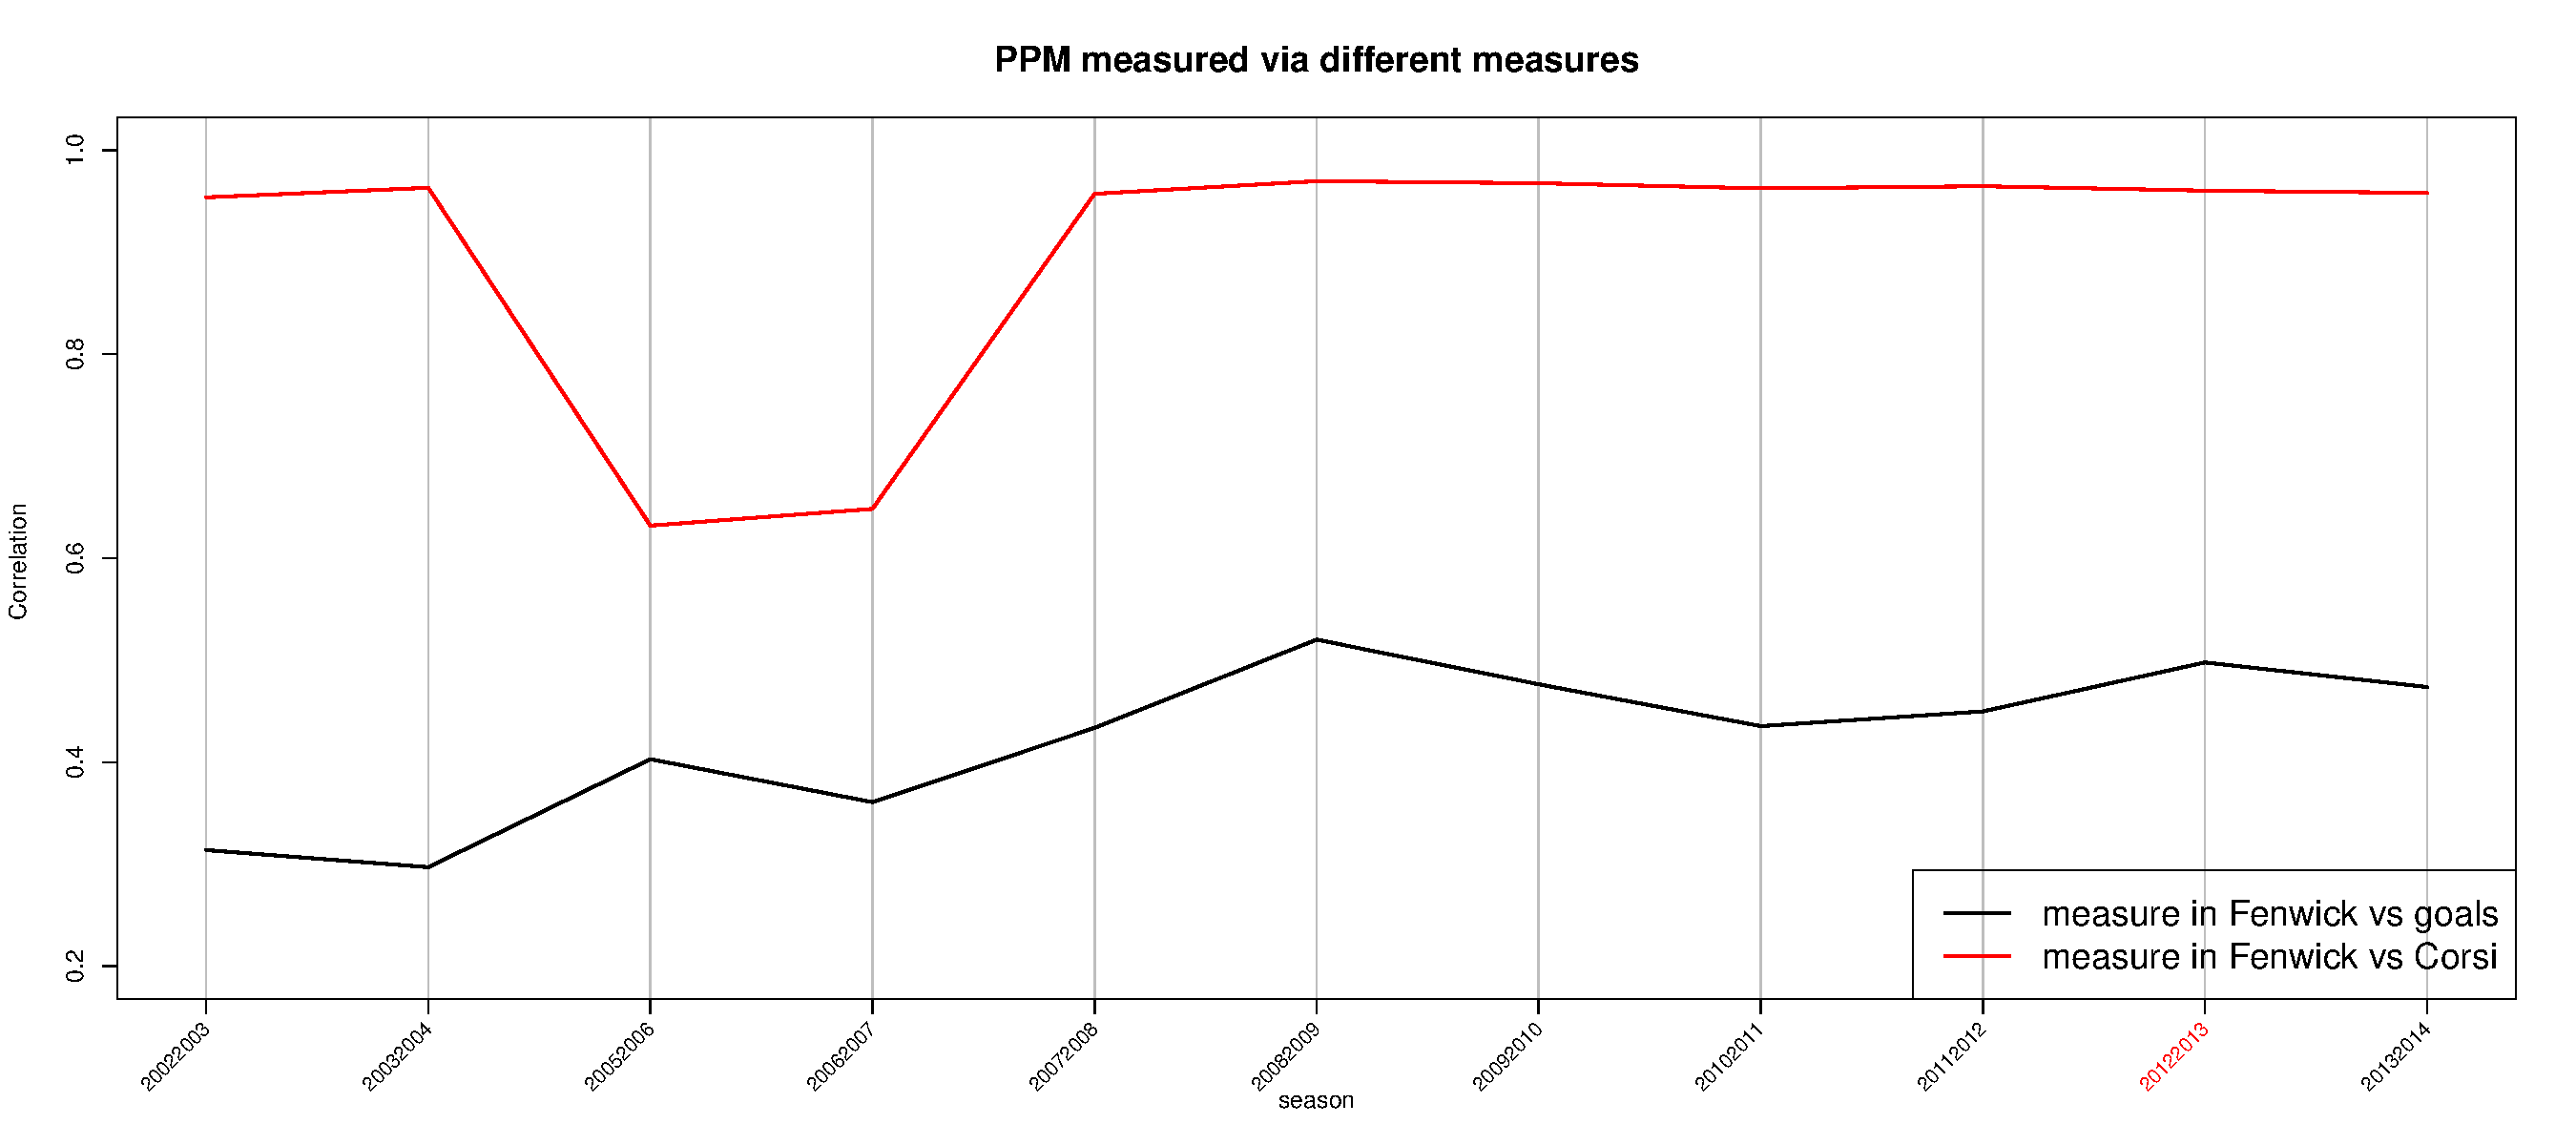
\includegraphics[width=\textwidth]{figures/ppm-corr-diffmeasure-season.pdf}
    \caption{Black: correlation of PPM measure in Fenwick and in goals over 11 seasons.  Red: correlation of PPM measure in Fenwick and in Corsi over 11 seasons.}\label{fig:ppm-corr-diffmeasure-season}
\end{figure}

\subsection{Value of players}
%%% code:  salary_sen.R

\begin{enumerate}
    \item Figure \ref{fig:ppmsal-corr-season}: PPM in goals is overall more correlated with salaries. All 3 lines show a decrease after lockout season 2004-2005. As to the 2013-2013 lockout, Corsi/Fenwick shows a drop in the correlation while goals shows a drop in the season after. Note Corsi even gives negative correlations for season 2006-2007 and 2005-2006. 
    \item Figure \ref{fig:ppmsal-scat}: Two measures are pretty consistent with each other. Sidney Crosby, Zach Parise and Ryan Suter are three most expensive players in season 2013-2014. According to our evaluation, both goals and Corsi show that Sidney Crosby is under paid while Ryan Suter is over paid. 
    \item Figure \ref{fig:salaryhist}
\end{enumerate}

\begin{figure}[htb!]
    \centering
    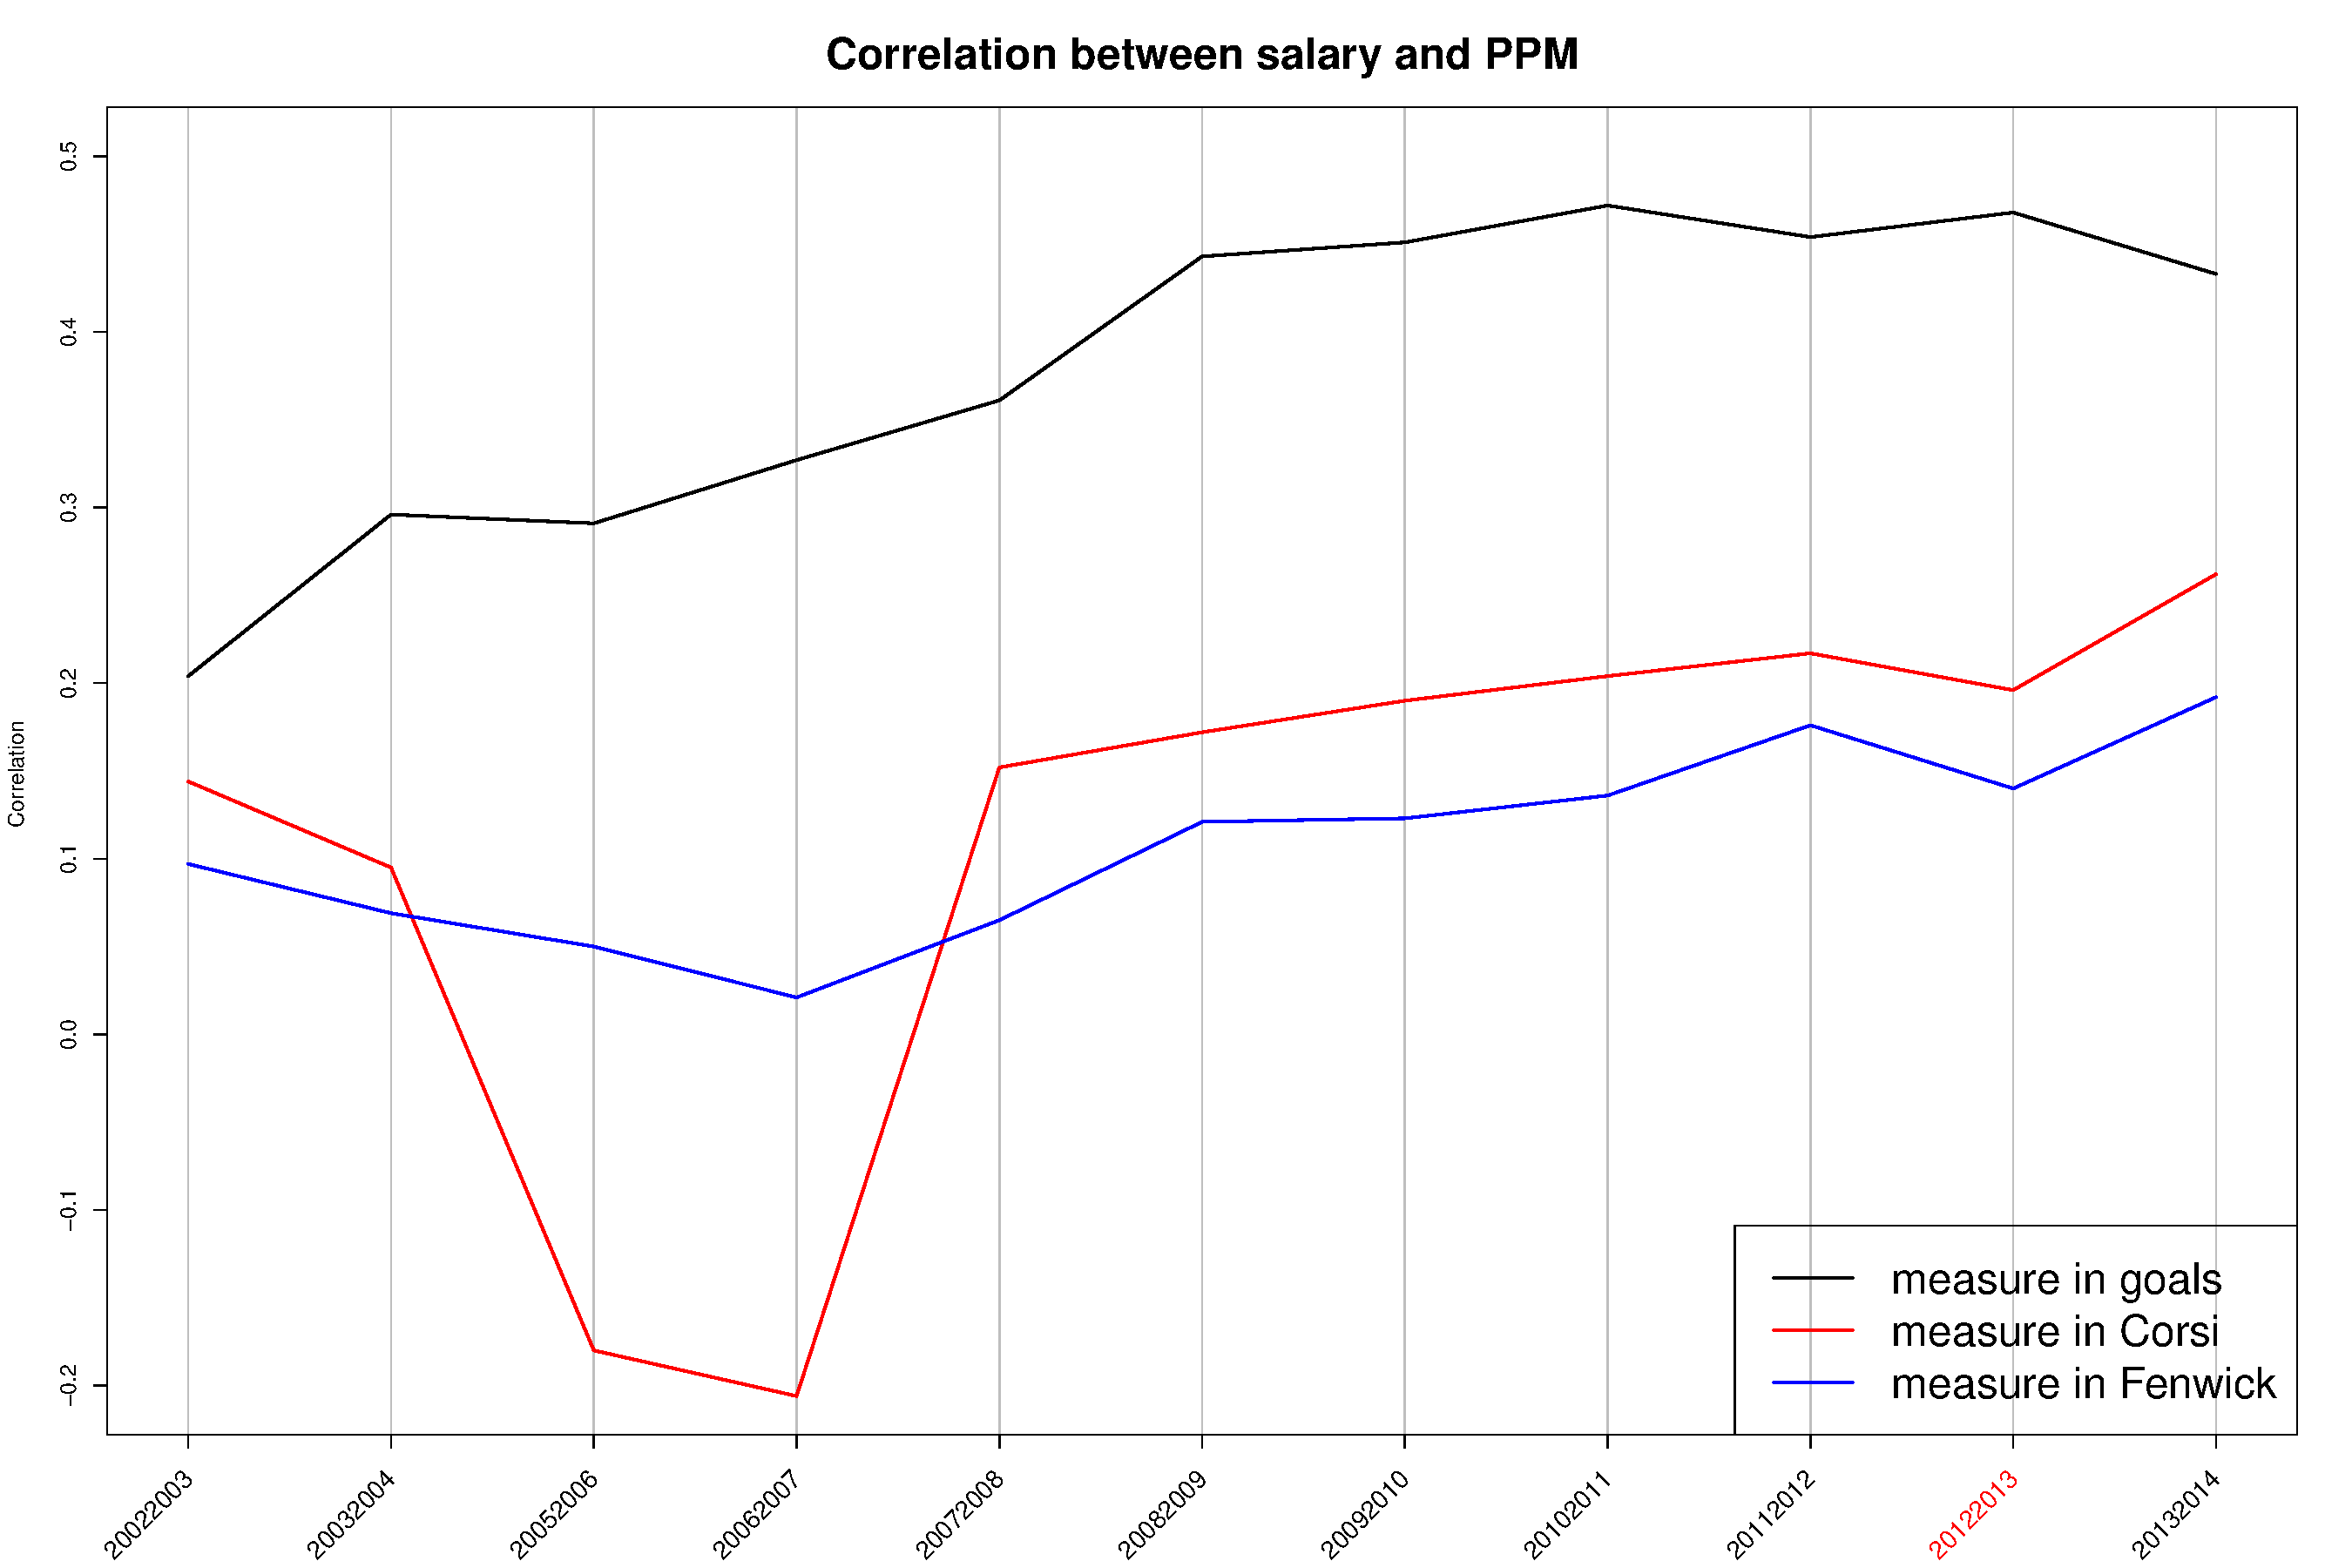
\includegraphics[width=0.8\textwidth]{figures/ppmsal-corr-season.pdf}
    \caption{Correlation between salary and PPM over 11 seasons with the lockout season 2012-2013 marked in red.}\label{fig:ppmsal-corr-season}
\end{figure}

\begin{figure}[htb!]
    \centering
    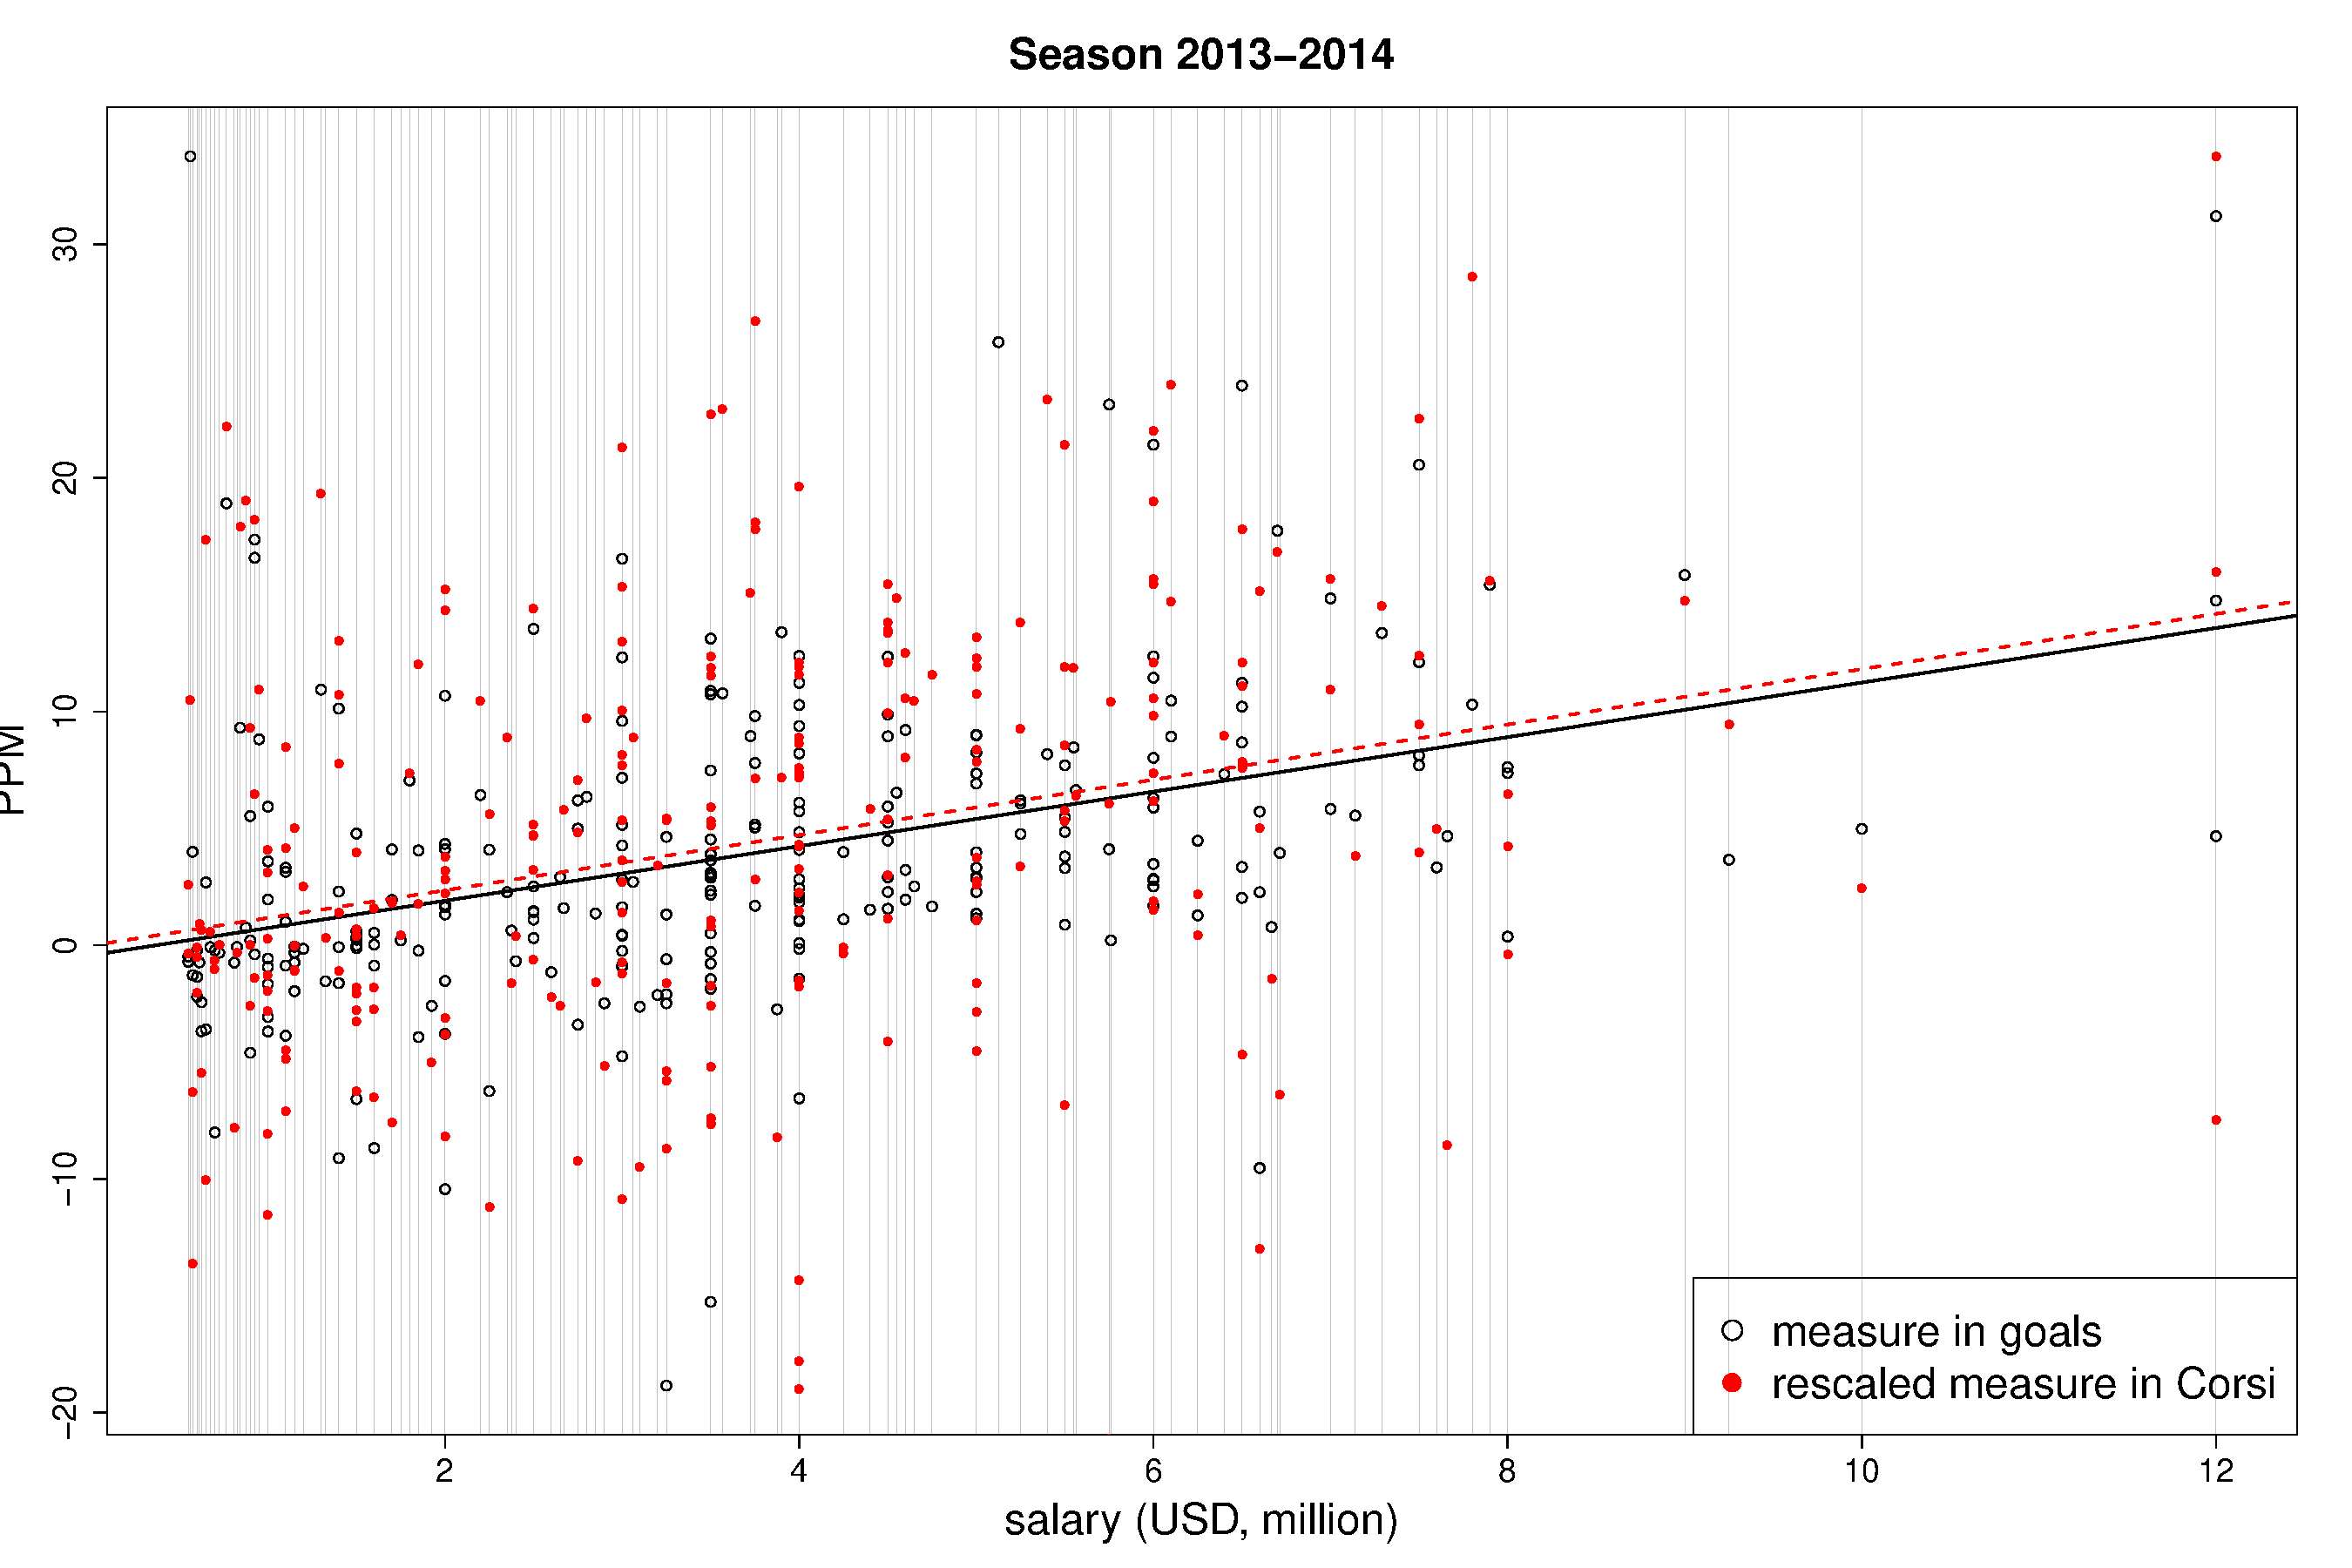
\includegraphics[width=0.8\textwidth]{figures/ppmsal-scat.pdf}
    \caption{Non-zero PPM via goals versus 2013-2014 salary, augmented with rescaled PPM via Corsi. Ordinary least squares fits are added to aid in visualization.}\label{fig:ppmsal-scat}
\end{figure}

\section{Analysis: the relationship between salary and performance}
\label{sec:salary}


\begin{figure}[htb!]
	\centering
	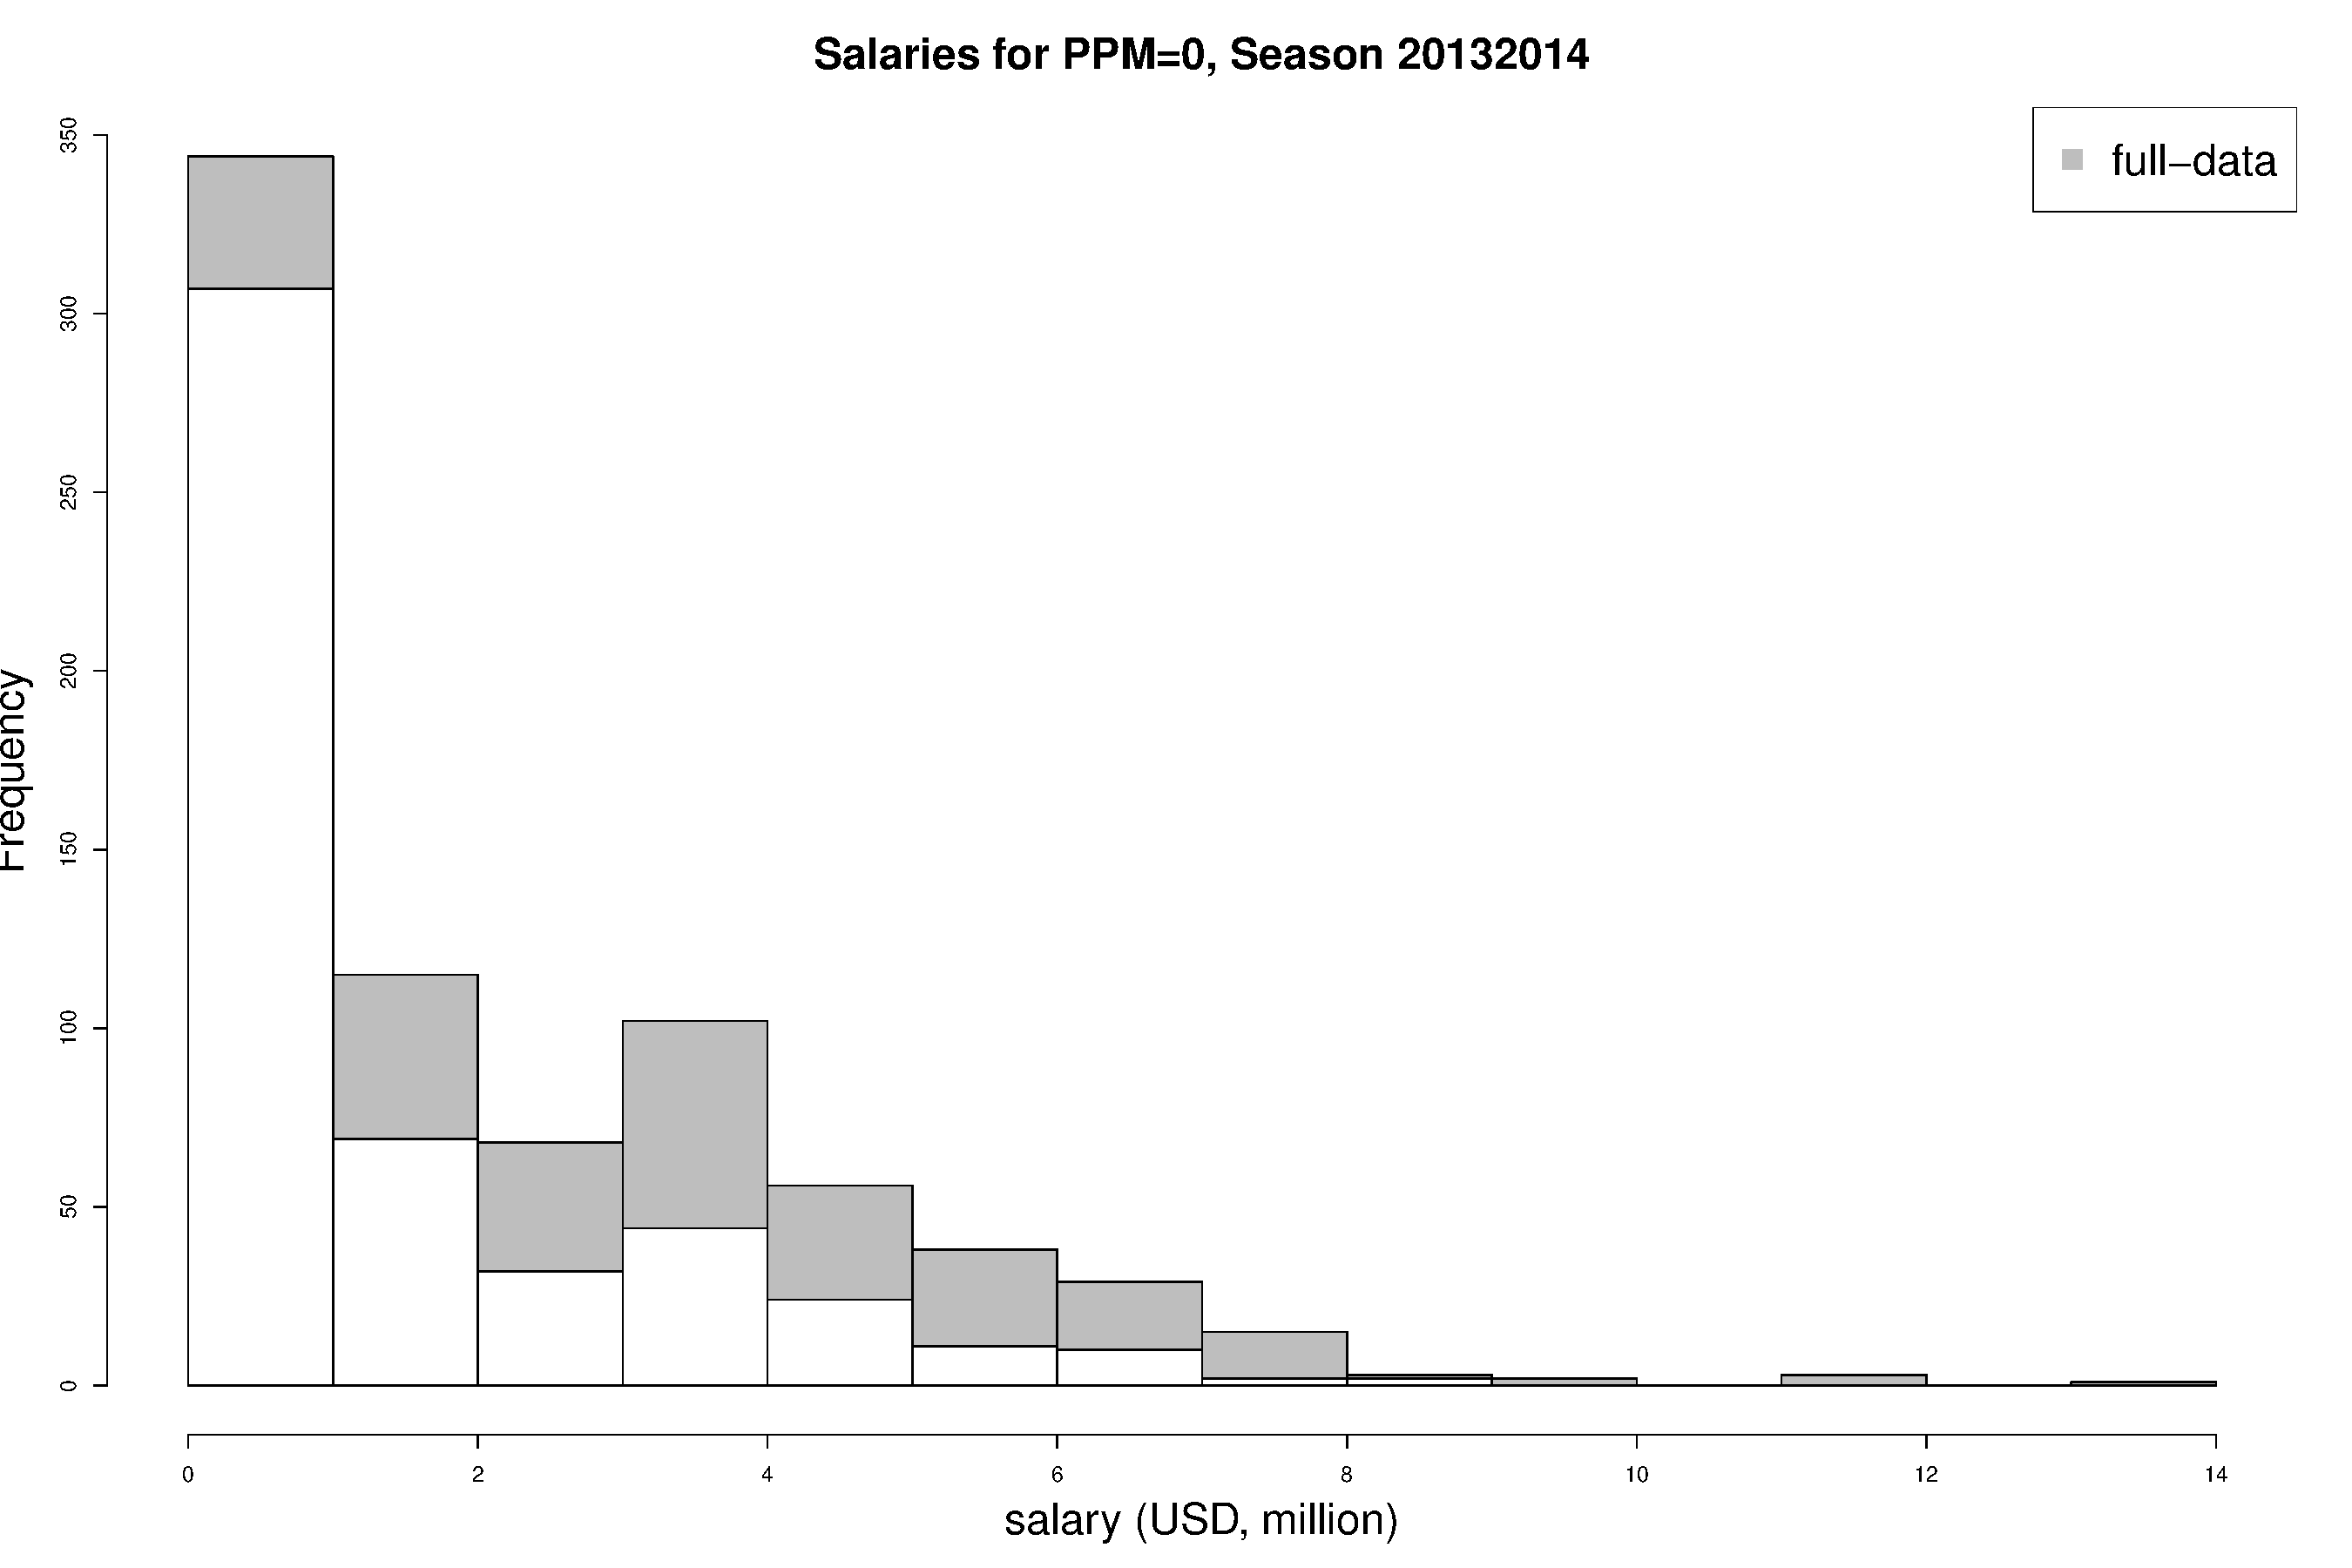
\includegraphics[width=0.8\textwidth]{figures/salaryhist.pdf}
	\caption{Histogram of 2013-2014 salaries for players with non-zero PPM exteading to the full set in gray.}\label{fig:salaryhist}
\end{figure}


\section{Conclusion}\label{sec:conclusion}

We have provided a sketch for how modern techniques in regularized logistic
regression, developed originally to address challenging large-scale problems
in genetics, finance, text mining, can be used to calculate partial player
effects in hockey.  We have argued that that such such partial effects are a
better measure of player ability compared to the classic plus-minus statistic,
and have the benefit of being interpretable on the same scale as plus-minus.
Our development has focused on point-estimation via the {\tt gamlr} package,
which infers parameters under L1 penalization.  Although there are other
software packages offering similar features, for example {\tt glmnet}
\cite{zou_regularization_2005}, we believe that {\tt gamlr} is particularly
well-suited to the data arizing in our hockey analysis, e.g., exploiting the
sparse structure of design matrices comprised of indicators where only a
handful (usually twelve) of thousands (of player) are nonzero. We have shown
how the framework is flexible, allowing one to control for many aspects of
situational play (special teams, overtime, playoffs), and personnel/season
(coaches, salaries, season-years).  A comparison was provided to the popular
Corsi and Fenwick alternatives to plus-minus, and we argued that a recent
emphasis in the literature on shots (and blocked shots), does not in general
compare favorably to the traditional goals focus in this framework.

Beyond model specification, there are several dimensions along which these
methods can be extended or generalized.  One is to break out of the
point-estimation context to apply a fully Bayesian analysis. The framework
originally suggested \cite{gramacy:jensen:taddy:2013} calculated a fully
Bayesian partial player effect via the {\tt reglogit} package for {\sf R},
implementing a Gibbs sampling strategy
\cite{gem:gem:1984} described in full by \cite{gra:pols:2012}.  It combines
two scale-mixture of normals data-augmentation schemes, one for the logit
\cite{holmes:held:2006} and one for the Laplace prior \cite{park:casella:2008}.
Obtaining $T$ samples from the full posterior, is straightforward using the
following {\sf R} code
\begin{verbatim}
bfit <- reglogit(T=T, y=Y, X=X, normalize=FALSE)
\end{verbatim}
The full posterior sample for $\beta$ residing in {\tt bfit} allows posterior
means to be calculated, as well as component-wise variances and correlations
between $\beta_j$'s.  \cite{gramacy:jensen:taddy:2013} show how these can be
used to, say, calculate the probability that one player is better than
another, rank them and provide posterior credible intervals for those
rankings\footnote{see., e.g, 
\url{https://github.com/TaddyLab/hockey/blob/master/results/blog/logistic_pranks_betas.csv}
} or be used to construct teams of players under budget constraints and
subsequently describe the probability that those teams will score more goals
than their opponents.  Like {\tt gamlr}, the software takes advantage of
sparse matrix libraries ({\tt slam} \cite{slam}), and is multi-threaded via
{\tt OpenMP} meaning it can multiple processors simultaneously, which is a
common configuration for modern desktop architectures. However, {\tt reglogit}
is still relatively slow when $n_p$ and $n_g$ are large, requiring several
hours to obtain thousands of samples from the posterior.

Another dimension for extension involves breaking out of the linear framework
entirely.  Anecdotally, we hear that some folks in the sports analytics
community (not just in hockey) prefer a framework built around random forests
\cite{breiman:2001}.  An advantage of trees, on which random forests are based,
is that they naturally explore (non-linear) interactions between predictors,
and thus players and other effects in the hockey analysis.  They also naturally
regularize and provide variable selection features via relevance statistics.  
A disadvantage is that the ensemble tree approach random forests provides does
not readily have a fully Bayesian interpretation, although recent work has 
shown that the ensemble can be seen to be approximating a Bayesian posterior
quantity \cite{taddy:eta:2015}.  Another option along similar lines is Bayesian
additive regression trees (BART, \cite{ChipGeorMcCu2010}), with newer visions
implemented non-linear logistic modeling via the same latent variable
techniques as in the linear case \cite{gra:pols:2012}.

In closing, we remark that it is easy to find flaws in our approach to
estimating partial player effects.  For example, although counting goals
measures time in some sense, the analysis does not directly utilize
time-on-ice information.  A similar drawback would exist for methods which are
instead tailored to shots, etc..  A method based on proportional hazards
\cite{ThoVenJen12}, however, does not suffer this drawback, as it incorporates
time-on-ice directly.  Nevertheless, the linear-logistic approach has much
to recommend it, including simple interpretation, easy extension in terms
of modeling framework and specification of predictors, and fast inference
so that player ability metrics and rankings are easily updatability when
new goals data arrive, making near-real-time analysis possible as games
and seasons progress.

\bibliographystyle{plain}
\bibliography{hockey}